% TODO(author) - confirmar antes de submeter:
% 1. Solow: coeficientes negativos (ex.: -2.31) com sum_equal_one=1 no codigo -> explicar como sao obtidos.
% 2. Solow: variavel 'rnna' (estoque de capital) usada no lugar de I/Y; confirmar redacao.
% 3. Solow: g+delta (0.03 nos apps 1-2; 0.05 no app 3) -> confirmar o que vale para os dois exercicios do paper.
% 4. Simulacoes dinamicas (exp. 9-12): parametros (NAS, lr, epocas) nao foram conferidos contra os scripts.
% 5. Numero de trials (1.000) nao conferido contra o codigo.
% 6. Tabelas Spearman e Top-K Rank: celulas identicas entre metodos (ex. IG/DL) -> checar.
% 7. Sem baseline OLS nas simulacoes; sem testes pareados.
% 8. Compilar com sn-jnl e .bib reais (nao foi possivel aqui).
\documentclass[preprint,12pt,authoryear]{sn-jnl}
\usepackage[utf8]{inputenc}
\usepackage[T1]{fontenc} 
\usepackage{natbib}
\usepackage{amsfonts,amsmath,amssymb,amsthm}
\usepackage{mathtools}
\usepackage[thinc]{esdiff}
\usepackage{multirow}
\usepackage{appendix}
\usepackage{tikz}
\usepackage{graphicx}
\usepackage{comment}
\usepackage{color,xcolor}
\usepackage{hyperref}
\usepackage{colortbl}
\usepackage{siunitx}
\usepackage{adjustbox}
%\usepackage{authblk}
\usepackage{csquotes}
\usepackage{subcaption}
\usepackage[capposition=top]{floatrow}
\usepackage{algpseudocode}
\usepackage{pdflscape}
\usepackage{booktabs}
\usepackage{setspace}
\usepackage{geometry}
\usepackage{enumitem}
\usepackage{iftex}

% Math Definitions
\newtheorem{lemma}{Lemma}
\newtheorem{proposition}{Proposition}
\newtheorem{theorem}{Theorem}
\newtheorem{corollary}{Corollary}
\newtheorem{definition}{Definition}
\newtheorem{research}{Research Question}
\newtheorem{property}{Property}
\newtheorem{remark}{Remark}

% Section with Extra Content
\newcommand{\sectionlabel}{Appendix}
\begin{document}

% ============================================================
% TITLE
% ============================================================

\title{Elasticity Decomposition in Cobb–Douglas Neural Networks}

% ============================================================
% AUTHORS
% ============================================================

\author*[1]{%
    \fnm{Jeronymo Marcondes} \sur{Pinto}%
}

\email{jeronymomp@gmail.com}

\author[2]{%
    \fnm{Martha Regina Meira} \sur{Bianchi}%
}

\email{martharmbianchi@gmail.com}

% ============================================================
% AFFILIATIONS
% ============================================================

\affil*[1]{%
    \orgname{Brazilian Ministry of Economics},
    \orgaddress{%
        \street{Esplanada dos Ministérios, Bloco F},
        \city{Brasília},
        \postcode{70059-900},
        \state{DF},
        \country{Brazil}
    }
}

\affil[2]{%
    \orgname{Federal University of São Paulo},
    \orgaddress{%
        \street{Rua Oleska Winogradow, 100},
        \city{Osasco},
        \postcode{06120-042},
        \state{SP},
        \country{Brazil}
    }
}

% ============================================================
% ABSTRACT
% ============================================================

\abstract{%
This paper proposes a neural network architecture grounded in
Input--Output economic systems, designed to provide intrinsic
structural interpretability. Unlike prevailing approaches that
treat interpretability as a post-processing step, the proposed
framework builds on product-unit networks and embeds economic
structure directly within the network: node exponents are
production elasticities, the elasticity of the output with respect
to each input is obtained analytically as the product of layer-wise
elasticity matrices, and transmission mechanisms can be traced
along production paths. Because the composition of Cobb--Douglas
layers is log-linear, depth acts as a hierarchical parameterization
of the global elasticity structure rather than as additional
expressive capacity. The approach yields a structurally transparent system that,
in our experiments, recovers directional effects and relative parameter
importance under suitable data-generating processes, with prediction
errors no larger than those of standard feedforward networks in the
simulated designs. In the Solow application, the standard OLS estimator
is the benchmark: the Neural IOM reproduces its elasticities in the
log-linear textbook specification, whereas post-hoc attributions of a
conventional network do not. We show that the Cobb--Douglas
node satisfies regularity conditions usually required of an activation
function, and that its gradients are bounded on a restricted domain. To validate the architecture, we run simulation experiments with known
parameters (twelve designs, 1,000 trials each). We also illustrate the
model in two applications to cross-country data from the Penn World
Table, based on the textbook and augmented Solow specifications of
\citet{mankiw1992contribution}. Code is available on
GitHub to ensure full reproducibility.
}

% ============================================================
% KEYWORDS
% ============================================================

\keywords{%
Neural Networks \sep
Input--Output Systems \sep
Cobb--Douglas Production \sep
Explainable AI \sep
Economic Networks
}

% ============================================================
% TITLE PAGE
% ============================================================

\maketitle

% ============================================================
% DECLARATIONS
% ============================================================

\section*{Declarations}

\subsection*{Competing Interests}

The authors declare that they have no competing interests.

\subsection*{Funding}

This research did not receive any specific grant from funding
agencies in the public, commercial, or not-for-profit sectors.

\subsection*{Data Availability}

The complete codebase and results are publicly available at
\url{https://github.com/jeronymomp/neural_cge_network}.

\subsection*{Declaration of Generative AI and AI-Assisted Technologies
in the Writing Process}

During the preparation of this work, the authors used AI-assisted
tools for grammar checking and language editing. After using these
tools, the authors reviewed and edited the content as needed and
take full responsibility for the content of the published article.

% ============================================================
% TITLE PAGE
% ============================================================



% ============================================================
% DECLARATIONS
% ============================================================


\onehalfspacing

% Section 1 - Introduction
\section{Introduction} \label{sec:introduction}

According to \cite{imbens2024causal}, understanding the structural parameters of an economic system is fundamental for policy design and economic analysis. Economic analysis aims not only to predict outcomes but to identify economically meaningful parameters such as elasticities and transmission coefficients.

At the same time, Economics has experienced a substantial increase in the adoption of artificial intelligence and machine learning methods \citep{zheng2023deep}, particularly deep learning. Owing to their high predictive accuracy, these systems approximate complex functional relationships and achieve state-of-the-art results in prediction and forecasting tasks \citep{dell2025deep}.

A central limitation of standard deep learning models is their \textbf{black-box} nature \citep{csahin2025unlocking}, which often prioritizes statistical correlation over theoretical consistency. From an economic perspective, this opacity hinders the ability to determine the dynamics of how individual covariates influence the output.

Many studies address the lack of structural interpretability of neural networks by introducing new methods or architectures to mitigate this issue. While some works focus on developing new theories based on models that explain the internal structure of neural networks, the majority remain model-agnostic, analyzing the effects of perturbing covariates on outputs without explicitly modeling the underlying dynamics \citep{molnar2020interpretable}. Throughout this paper, interpretability refers to intrinsic structural transparency as the analytical propagation of elasticities and the recovery of directional effects—rather than causal identification in the econometric sense.

This study proposes a neural network architecture that emulates a production network, where each neuron acts as a firm and its output is equivalent to the neuron's activation, inspired by the Input–Output Model (IOM) \citep{leontief1986input}. We adopt a Cobb–Douglas production function as the activation mechanism. While this imposes a specific functional structure, it is particularly suited for modeling economic systems where multiplicative interactions and constant elasticities are theoretically plausible. By doing so, we obtain a parameterization in which input elasticities and transmission effects are structurally coherent and analytically traceable.

We develop an economic-inspired neural network architecture, grounded in \cite{leontief1986input}, designed to provide intrinsic structural interpretability. By embedding a Cobb-Douglas functional form, the framework enables the analytical propagation of cumulative elasticities, allowing us to quantify how local contributions propagate to global outputs across successive layers. We show that the Cobb--Douglas node satisfies the regularity conditions of an admissible activation function, make explicit that the resulting composition is log-linear (so that depth parameterizes, rather than enlarges, the function class), and evaluate it in simulations with known ground truth and in the Solow model. The aim is not to outperform standard econometric estimators: where the specification is log-linear, as in the Solow application, OLS is the benchmark, and the question is whether a neural parameterization can reproduce its elasticities while remaining a neural network. Post-hoc attributions of a conventional network, by contrast, do not deliver elasticities. The resulting system is structurally transparent and, under suitable data-generating processes, recovers directional effects, relative importance and structural parameters.

\subsection{Research Gap}
The Neural IOM is closely related to the broader literature on multiplicative and product-unit neural networks. Product units were introduced as an alternative to conventional additive neurons, replacing weighted summation by multiplicative interactions of the form

$$
z=\prod_{j=1}^{p}x_j^{w_j},
$$

where the weights operate as exponents rather than as multiplicative coefficients \citep{durbin1989product}. Subsequent work has developed product-unit neural networks (PUNNs) for regression, classification, and other nonlinear prediction tasks, emphasizing their ability to represent higher-order interactions and nonlinear relationships with relatively compact architectures. \citep{bas2016training}

The basic computational similarity with the Neural IOM is therefore direct: both approaches use multiplicative transformations in which input variables are raised to learned powers. The distinction of the Neural IOM lies instead in the \textbf{economic structure imposed on these multiplicative operations and in the interpretation of their parameters}. Product-unit networks are generally developed as flexible nonlinear approximators, with the exponents serving primarily as parameters governing the shape of the approximation. In the Neural IOM, the exponents are interpreted as production elasticities, while successive Cobb--Douglas transformations are organized as an input-output network. Consequently, the network represents a sequence of economically interpretable production transformations rather than simply a collection of multiplicative basis functions.

This structure also changes the interpretation of parameters beyond the individual product unit. Because the output of one Cobb--Douglas node can enter subsequent nodes, an input can affect the final output through multiple production stages. The resulting effect is therefore not necessarily identified with a single exponent in one multiplicative unit. Instead, the architecture permits the construction of \textbf{cumulative economic effects through the network}, which can be interpreted in terms of elasticities propagated along production paths. 

Thus, the contribution of the Neural IOM is not the introduction of multiplicative neurons per se. Rather, it is the use of a well-established multiplicative neural-network mechanism to construct a network whose computational parameters have a direct interpretation within an input-output production system. This distinction is particularly relevant for economic applications, where the objective is not only nonlinear prediction but also the recovery and interpretation of economically meaningful relationships among inputs, intermediate outputs, and final production.

To the best of our knowledge, product-unit networks have not previously been organized and read as elasticity-propagating input--output systems for the purpose of interpretability. The contributions of the paper are therefore the following:

\begin{enumerate} [leftmargin=*, itemsep=0pt, topsep=2pt, parsep=0pt]
    \item an architecture in which the elasticity of each output with respect to each input is extracted analytically, as the product of layer-wise elasticity matrices, and can be decomposed along production paths (Property \ref{prop:elasticity});
    \item an explicit statement of the scope of this construction: the composition is log-linear, so depth is a hierarchical parameterization of the elasticity structure rather than a source of additional expressive capacity (Remark \ref{rem:collapse});
    \item a large-scale Monte Carlo comparison, with known ground truth, of the recovery of directional effects by the Neural IOM and by post-hoc attribution methods applied to standard feedforward networks; and
    \item an application to the Solow model in which OLS is the benchmark: the elasticities extracted from the Neural IOM are compared with OLS estimates and, in turn, with post-hoc attributions of a standard feedforward network.
\end{enumerate}

The remainder of the paper is organized as follows. Section \ref{sec:research_problem} formulates the research problem, highlighting the lack of structural transparency and directional traceability in standard neural networks. Section \ref{sec:theory} develops the theoretical intuitions of the proposed framework. Section \ref{sec:simulation} presents a large-scale Monte Carlo study, comprising 12,000 experiments, to evaluate performance in a controlled setting. Section \ref{sec:solow} provides an empirical application using cross-country panel data from the Penn World Table, replicating two classical specifications of \cite{mankiw1992contribution}: the textbook Solow model and the human-capital augmented specification. This section also includes empirical comparative statics exercises to illustrate the model's structural responses. The final section concludes.

\section{Research Problem: Neural Network as a Black Box} \label{sec:research_problem}

\textit{The central limitation of feedforward neural networks in economic applications is not predictive accuracy, but the absence of intrinsic structural transparency and the lack of analytical traceability regarding how covariates dynamically influence the output}. The literature on the interpretability of Neural Networks can be broadly divided into two strands: model-based approaches and model-agnostic (post-hoc) methods.

Model-based approaches seek to open the “black box” by redesigning neural architectures to enhance transparency. Examples include additive decompositions, structured component models, and causality-inspired architectures \citep{yang2021gami, wu2025explainable, cho2024deep}. Other contributions interpret trained networks using tools from Random Matrix Theory or algebraic topology \citep{martin2021implicit, spannaus2024topological}. While these approaches introduce useful structural constraints, the discussion on the interpretability of Neural Networks is far from concluded.

Model-agnostic methods, by contrast, treat neural networks as black boxes. Techniques such as Shapley values and gradient-based attributions quantify feature relevance by perturbing inputs and observing changes in predictions. Formally, Shapley values ($SHAP$) assign to each feature its average marginal contribution across all possible coalitions:

\begin{equation}
\phi_j(\text{val}) = \sum_{S \subseteq \{1,\dots,p\}\setminus\{j\}} 
\frac{|S|!(p-|S|-1)!}{p!} \Big(\text{val}(S \cup \{j\}) - \text{val}(S)\Big).
\end{equation}

The Shapley value $\phi_j(\text{val})$ represents the permutation-weighted average marginal contribution of feature $j$ across all possible subsets $S$ out of $p$ total features, where $\text{val}(S)$ evaluates the model's output for a given coalition.

In addition to Shapley values, several other agnostic methods have been developed to enhance the interpretability of neural networks. These include \textbf{Integrated Gradients} ($IG$), which integrates the gradients of the model’s output with respect to its inputs for a given baseline \citep{sundararajan2017axiomatic}; \textbf{Noise Tunnel} ($NT$), which introduces a perturbation into an attribution method (here Integrated Gradients) and evaluates the final impact \citep{smilkov2017smoothgrad}; \textbf{DeepLIFT} ($DL$), which decomposes the target prediction by backpropagating the contribution of all neurons with respect to each feature, allowing a comparison of activations before and after the process \citep{shrikumar2017learning}; \textbf{Gradient SHAP} ($GS$), which samples multiple input baselines, adds Gaussian noise to the inputs, and applies Integrated Gradients to each perturbed sample, averaging the attributions to approximate SHAP values \citep{kokhlikyan2020captum}; and \textbf{Feature Ablation} ($FA$), which defines baseline values for features (e.g., setting them to zero) and measures the variation in model output when other features are altered \citep{molnar2020interpretable}.

Although informative at the level of individual predictions, these methods are inherently local and ex-post: they approximate the model's behavior in the neighborhood of a single observation without ensuring theoretical consistency in the direction of the effects across the global distribution. As a result, they offer limited insight into the underlying structural mechanisms that drive aggregate economic dynamics. This raises a fundamental research question:

\begin{research} \label{research_question}
    \textit{Can a feedforward neural network be represented as a system in which variations in covariates generate analytically traceable directional dynamics and cumulative effects on the final output, in the form of elasticities that can be extracted from the estimated parameters and decomposed along economic-founded interpretable transmission channels}?
\end{research}


\section{Theoretical Insights} \label{sec:theory}

This work proposes a feedforward neural network architecture that emulates a nonlinear input--output production system. By establishing a formal correspondence between feedforward neural networks and input--output models (IOMs), and by specifying Cobb--Douglas production functions at each node, the resulting architecture provides intrinsic structural transparency, enabling the analytical propagation of cumulative elasticities and the tracing of transmission mechanisms across layers \citep{acemoglu2012network}.

The theoretical development proceeds in two steps. First, we show the structural correspondence between IOMs and neural networks under a directed acyclic graph (DAG) representation. Second, we characterize the multiplicative propagation of elasticities induced by the Cobb--Douglas specification and establish the conditions under which this representation is well-defined and numerically stable. Importantly, although each layer is nonlinear in the original input space, its logarithmic representation is linear. This property makes the cumulative elasticity structure analytically tractable.


\subsection{Conceptual Correspondence between Neural Networks and the IOM}

Both input–output models and feedforward neural networks admit representation as weighted directed graphs \citep{sargent2024economic}. In an IOM, vertices correspond to productive units (firms or sectors), while edges represent flows of inputs weighted by technical coefficients. In a feedforward neural network, vertices correspond to neurons, edges correspond to weighted linear transformations, and nonlinear activation functions operate at each node within an acyclic layered structure.

Suppose that the productive structure of an economy is described according to equation \ref{iom matrix}. Traditional IOMs allow feedback flows of inputs and outputs circulating among firms in the economy. However, when the production structure is acyclic, the IOM can be interpreted as a directed acyclic graph, where nodes represent productive units and edges capture the flows of intermediate goods between them. In this representation, the elements $z_{ij}$ of the input–output matrix $Z$ denote the quantity of output from sector $i$ required as input by sector $j$, and the adjacency matrix corresponds to the weighted matrix of inter-sectoral flows.

\begin{equation} \label{iom matrix}
\setlength{\abovedisplayskip}{5pt}
\setlength{\belowdisplayskip}{5pt}
\mathbf{x} = \mathbf{Z}\mathbf{i} + \mathbf{f}, \quad 
\mathbf{x} = 
\begin{bmatrix} x_1 \\ \vdots \\ x_n \end{bmatrix}, \;
\mathbf{Z} = 
\begin{bmatrix} z_{11} & \cdots & z_{1n} \\ \vdots & \ddots & \vdots \\ z_{n1} & \cdots & z_{nn} \end{bmatrix}, \;
\mathbf{f} = 
\begin{bmatrix} f_1 \\ \vdots \\ f_n \end{bmatrix}.
\end{equation}

Feedforward neural networks (FNNs) are likewise directed acyclic graphs (DAGs) in which information flows from inputs to outputs through successive layers \citep{sargent2024economic}. Formally, an FNN can be represented as a composition of affine transformations and activation functions:

\begin{equation} \label{fnn_equation}
\Phi(x) = (\sigma \circ T_L \circ \sigma \circ T_{L-1} \circ \cdots \circ \sigma \circ T_1)(x),
\quad \text{where } T_\ell(x) = W_\ell x + b_\ell.
\end{equation}

In this sense, the depth of the network ($L$) corresponds to the number of production stages, representing a structural dynamics in which inputs are iteratively transformed into higher-order intermediate goods. The layered composition in \eqref{fnn_equation} mirrors the sequential transformation of intermediate outputs across production stages. Under an acyclic structure, both systems define ordered transformations in which weighted connections govern how intermediate quantities propagate toward a final outcome. This can be visualized in the Figure \ref{fig:simple_dag}.


\begin{figure}[htbp]
\centering
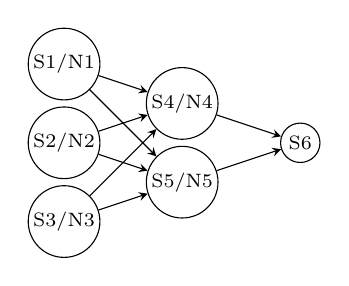
\begin{tikzpicture}[x=1.5cm, y=1cm, >=stealth, every node/.style={circle, draw, minimum size=5mm, inner sep=1pt, font=\scriptsize}]

% Nodes
\node (S1) at (0,2) {S1/N1};
\node (S2) at (0,1) {S2/N2};
\node (S3) at (0,0) {S3/N3};

\node (H1) at (1,1.5) {S4/N4};
\node (H2) at (1,0.5) {S5/N5};

\node (O1) at (2,1) {S6};

% Connections
\foreach \s in {S1,S2,S3} {
    \foreach \h in {H1,H2} {
        \draw[->] (\s) -- (\h);
    }
}
\foreach \h in {H1,H2} {
    \draw[->] (\h) -- (O1);
}

\end{tikzpicture}
\caption{DAG representing Analogy Between IOM and FNN.}
\label{fig:simple_dag}

{\scriptsize Note: S1--S3 are input sectors/neurons, S4--S5 hidden sectors/neurons, and S6 the output sector/neuron.}
\end{figure}

\begin{definition}[Neural Network as an IOM] \label{def:nn_as_iom}
In the absence of feedback loops, an IOM admits a strictly layered representation. Let $x^{(0)} \in \mathbb{R}^d$ and define

$$
x^{(\ell)} = \phi^{(\ell)}(W^{(\ell)}x^{(\ell-1)}),
\quad \ell = 1,\dots,L.
$$

This structure is equivalent to a feedforward neural network and induces a mapping
$F:\mathbb{R}^d\to\mathbb{R}^k$ given by

$$
F =
\phi^{(L)}\circ W^{(L)}
\circ\cdots\circ
\phi^{(1)}\circ W^{(1)}.
$$

When the node transformation is specified by a Cobb--Douglas function, the resulting mapping is multiplicative in the original input space and admits a linear representation in logarithmic coordinates. The layered structure therefore provides a convenient parameterization for tracing how input elasticities are transmitted across production stages.
\end{definition}


\subsection{The Proposed Neural IOM System}

Traditional IOMs often rely on Leontief production technology, which imposes fixed input proportions. Replacing this specification with a Cobb–Douglas production function introduces substitutability among inputs while preserving analytical tractability.\footnote{For more details on Cobb-Douglas production function and its properties, see \cite{sargent2024economic}.} In the proposed framework, each neuron implements a Cobb--Douglas-type transformation. Let $x \in \mathbb{R}^n_{+}$ and define

\begin{equation} \label{log_cobb_douglas_1}
y = \exp\left( \sum_{i=1}^n \alpha_i \ln x_i \right),
\end{equation}

where $\alpha_i$ denotes the output elasticity with respect to input $x_i$. This log-linear representation is equivalent to the standard Cobb--Douglas form and is compatible with layered compositions.

This expression is equivalent to the standard Cobb–Douglas formulation written in exponential log-linear form. The log representation aligns the multiplicative structure of the production function with the additive structure required for layered compositions, enabling analytical tracing of elasticity transmission across stages. This architecture follows the pattern proposed by \cite{bas2016training}.

Through training, the values of $\alpha_i$ are estimated. Consider a simplified network with $k$ layers, $n=1$ in each layer, and zero bias for exposition. Since $y_{1,k} = x_{1,k}^{\alpha_{1,k}}$ and $x_{1,k} = y_{1,k-1}$, recursive substitution yields:

\begin{equation} \label{cobb_douglas_composition}
y_{1,k} 
= \left( \cdots \left( \left( x_{1,1}^{\alpha_{1,1}} \right)^{\alpha_{1,2}} \right)^{\cdots \alpha_{1,k-1}} \right)^{\alpha_{1,k}}
= x_{1,1}^{\prod_{j=1}^{k} \alpha_{1,j}}.
\end{equation}

This result shows that the total elasticity of the final output with respect to the original input equals the product of the layer-specific elasticities. More generally, in vector form, elasticity propagation across layers can be represented as successive matrix multiplications:

\[
\mathbf{e}_j \longmapsto A^{(1)} \mathbf{e}_j \longmapsto A^{(2)} A^{(1)} \mathbf{e}_j \longmapsto \cdots \longmapsto A^{(L)} \cdots A^{(1)} \mathbf{e}_j,
\]

where $A^{(\ell)}$ denotes the matrix of elasticities in layer $\ell$. This recursive structure defines a propagation operator that is linear in logarithmic coordinates, whose cumulative effect is analytically tractable, providing both computational efficiency and structural interpretability. 

\begin{definition}[Neural IOM] \label{def:neural_iom}
Let $x \in \mathbb{R}^n_{+}$. A Neural IOM is a mapping $T: \mathbb{R}^n_{+} \to \mathbb{R}^m_{+}$ defined componentwise by
\[
T_k(x) = \exp\left( \sum_{i=1}^n \alpha_{ki} \ln x_i \right), \quad k = 1, \dots, m,
\]
where $\alpha_{ki} \in \mathbb{R}$ denotes the elasticity of output $k$ with respect to input $i$. The matrix $A = (\alpha_{ki})$ is called the elasticity matrix of the layer.
\end{definition}

The next result formalizes the extraction of elasticities, which is the central interpretability device of the framework.

\begin{property}[Global elasticities and path decomposition] \label{prop:elasticity}
Let $T^{(\ell)}$, $\ell=1,\dots,L$, be Neural IOM layers with elasticity matrices $A^{(\ell)}$, and let $T = T^{(L)}\circ\cdots\circ T^{(1)}$. Then, for every $x\in\mathbb{R}^n_{+}$:
\begin{enumerate} [leftmargin=*, itemsep=0pt, topsep=2pt, parsep=0pt]
    \item[(i)] $\ln T(x) = A \ln x$ with $A = A^{(L)}\cdots A^{(1)}$; hence $\partial \ln T_k(x)/\partial \ln x_i = A_{ki}$, a constant that does not depend on $x$;
    \item[(ii)] $A_{ki} = \sum_{\pi} \prod_{\ell=1}^{L} \alpha^{(\ell)}_{j_\ell j_{\ell-1}}$, where the sum runs over all paths $\pi = (i = j_0 \to j_1 \to \cdots \to j_L = k)$ through the network, so that each term is the contribution of one production path to the cumulative elasticity;
    \item[(iii)] if every $A^{(\ell)}$ has nonnegative entries and rows summing to one (constant returns to scale), so does $A$.
\end{enumerate}
\end{property}

\begin{proof}
(i) follows by induction: if $\ln y^{(\ell-1)} = A^{(\ell-1)}\cdots A^{(1)} \ln x$, then $\ln y^{(\ell)} = A^{(\ell)} \ln y^{(\ell-1)}$ by the definition of the layer. (ii) is the expansion of the matrix product into a sum over index sequences. (iii) A product of nonnegative matrices is nonnegative, and $A\mathbf{1} = A^{(L)}\cdots A^{(1)}\mathbf{1} = \mathbf{1}$.
\end{proof}

\begin{remark}[Depth as hierarchical parameterization] \label{rem:collapse}
By Property \ref{prop:elasticity}(i), a Neural IOM with $L$ layers (without additive terms between layers) represents exactly the same functions as a single Cobb--Douglas layer with elasticity matrix $A = A^{(L)}\cdots A^{(1)}$, that is, a log-linear model. Depth therefore does not enlarge the function class; it organizes the global elasticity matrix into economically interpretable production stages and enables the path-wise decomposition in Property \ref{prop:elasticity}(ii). The Neural IOM should accordingly be read as a neural parameterization of a constant-elasticity model rather than as a universal approximator. A log-linear regression estimated directly (e.g., by OLS) belongs to the same function class, which is why OLS is the natural benchmark in Section \ref{sec:solow}.
\end{remark}

\subsection{Cobb--Douglas as an Activation Function}

In the proposed architecture, the Cobb--Douglas function is used as a node-level transformation rather than as a conventional activation function in the sense of universal approximation theory. Its suitability for the Neural IOM follows from three properties that are directly relevant to the proposed application: non-linearity in the original input space, differentiability on the strictly positive domain, and a direct economic interpretation of its parameters as output elasticities.

The purpose of this section is not to establish a general or definitive result on the suitability of the Cobb--Douglas function as an activation function for arbitrary neural network architectures. Rather, we characterize the mathematical properties that motivate its use within the proposed Neural IOM framework. In particular, the Cobb--Douglas specification allows the parameters associated with individual input features to be interpreted directly as output elasticities, while retaining desirable regularity and numerical properties of a nonlinear node-level transformation. These characteristics are central to the structural interpretability of the proposed architecture and distinguish the role of the Cobb--Douglas function in the Neural IOM from that of a generic activation function whose primary purpose is to increase the expressive capacity of a neural network.

We therefore establish the relevant mathematical properties of the transformation and subsequently characterize the conditions under which its derivatives remain bounded. The results are intended to support the use of the Cobb--Douglas function as a structurally interpretable node-level transformation, rather than to establish universal approximation for the Neural IOM architecture or for arbitrary neural network architectures.


\begin{proposition}\label{proposition_1}
Consider the Cobb--Douglas function defined in equation \ref{log_cobb_douglas_1}. Then: (i) it is non-linear; (ii) it is differentiable; and (iii) it is well-defined for all strictly positive inputs.
\end{proposition}

\begin{lemma} \label{lemma_continuity}
The Cobb--Douglas activation function defined in equation \ref{log_cobb_douglas_1} is locally Lipschitz continuous.
\end{lemma}

\begin{lemma} \label{lemma_nonconstant}
The Cobb--Douglas activation function defined in equation \ref{log_cobb_douglas_1} is nonconstant.
\end{lemma}

The preceding results establish the regularity properties required for the mathematical and computational treatment of the proposed transformation. They do not, however, imply universal approximation for the complete Neural IOM architecture. In particular, because the logarithm of each Cobb--Douglas layer is a linear transformation, consecutive layers without biases or additional nonlinear operations collapse to a single linear transformation in logarithmic coordinates (Remark \ref{rem:collapse}). Hence, the depth of the present architecture does not enlarge the global function class in the manner of a conventional multilayer neural network.

This property is not a limitation for the structural objective of the Neural IOM. Rather, it implies that depth should be interpreted as a hierarchical parameterization of the global elasticity structure. The product of the layer-specific elasticity matrices determines the overall input--output elasticities, while preserving the economic interpretation of the underlying multiplicative mapping.

The following result is offered as an \emph{intuition} that the Cobb--Douglas transformation is a well-behaved nonlinear unit: it checks the regularity conditions (continuity, boundedness, non-constancy) usually invoked in Hornik-type approximation results. It is not used to claim universal approximation for the Neural IOM, and it does not extend to the depth-collapsed architecture described above. Hornik's theorem is stated for units applied to an affine combination of the inputs, so its literal application to a multi-input Cobb--Douglas node would require additional arguments that we do not pursue.

\begin{theorem}[Regularity of the Cobb--Douglas Node as a Candidate Activation Function] \label{theorem_1}
Consider the Cobb--Douglas function defined by equation \ref{log_cobb_douglas_1} used as a node-level transformation within a conventional layered architecture $\Phi(x) = (\sigma \circ T_L \circ \cdots \circ \sigma \circ T_1)(x)$ with linear combination at the output layer, as in equation \ref{fnn_equation}. Because this transformation is non-constant, continuous, and bounded on the domain $[\varepsilon,1]^n$ (Lemmas \ref{lemma_continuity}--\ref{lemma_nonconstant}), it satisfies the regularity conditions (continuity, boundedness, non-constancy) that Hornik-type approximation results require of an activation function. We read this as an indication that the transformation is an admissible candidate for node-level use within conventional architectures, not as a proof of approximation for any specific architecture; it does not extend to the depth-collapsed Neural IOM architecture of Definition \ref{def:neural_iom}, whose function class is discussed above.
\end{theorem}

Beyond admissibility, numerical stability is essential for any practical implementation. For the function in equation \ref{log_cobb_douglas_1}, we have:
\[
\frac{\partial y}{\partial x_i} = \frac{\alpha_i}{x_i}y.
\]
Gradient values may vanish or explode depending on the behavior of $x_i$ and $\alpha_i$. To ensure bounded derivatives and stable propagation, we impose the constraints $x_i \in [\varepsilon,1]$ (with $\varepsilon > 0$), $\alpha_i \geq 0$, and $\sum_{i=1}^n \alpha_i = 1$.

\begin{theorem}[Cobb--Douglas Activation Function Numerical Stability] \label{theorem_2}
Let $f$ be the Cobb-Douglas activation function defined by equation \ref{log_cobb_douglas_1}. Under the constraints $x_i \in [\varepsilon, 1]$, $\alpha_i \geq 0$, and $\sum_{i=1}^n \alpha_i = 1$, the partial derivatives satisfy $\left|\frac{\partial y}{\partial x_i}\right| \leq \frac{\alpha_i}{\varepsilon}$ and $\left|\frac{\partial y}{\partial \alpha_i}\right| \leq |\ln \varepsilon|$. Moreover, $\frac{\partial y}{\partial x_i} \geq \alpha_i \varepsilon$ whenever $\alpha_i > 0$. Hence gradients do not explode, and gradients with respect to the inputs that carry a positive elasticity do not vanish.
\end{theorem}

\begin{corollary}[Cobb-Douglas as a Valid Activation Function] \label{corollary}
Under the constraints $\varepsilon \leq x_i \leq 1$, $\alpha_i \geq 0$, and $\sum_{i=1}^n \alpha_i = 1$, the Cobb-Douglas function defined in equation \ref{log_cobb_douglas_1} constitutes a valid node-level activation function, as it satisfies: (i) non-linearity, differentiability, and well-definedness; (ii) the regularity conditions (continuity, boundedness, non-constancy) of Hornik-type results for node-level use within conventional architectures; and (iii) bounded gradient propagation. Within the Neural IOM architecture of Definition \ref{def:neural_iom}, however, the absence of nonlinear operations between layers (a bias enters only as a multiplicative constant) causes the composition to collapse to a single log-linear transformation, so depth serves as a hierarchical parameterization of elasticities rather than as a source of additional expressive capacity.
\end{corollary}

Under the stated domain and parameter restrictions, the Neural IOM architecture combines intrinsic structural transparency with a multiplicative functional form whose parameters admit a direct elasticity interpretation. The layered representation provides a hierarchical parameterization of these elasticities and allows their cumulative effects to be traced analytically from original inputs to final outputs. The resulting structure is therefore designed primarily for economically interpretable representation rather than for expanding the function class through depth.


\subsection{Economic Foundations and Constraints} \label{sec:economic_constraints}

The Neural IOM imposes two structural constraints derived from production theory: strictly positive inputs and constant returns to scale.

\textbf{Positive Domain}

Let $x \in \mathbb{R}^n$. To ensure that logarithmic transformations are well-defined, inputs are mapped into a strictly positive domain via $\tau: \mathbb{R} \to (\epsilon,1]$, with $\epsilon > 0$. A common choice for $\tau$ is a bounded monotonic map such as min--max normalization followed by clipping to $[\varepsilon,1]$, although the specific parametrization does not affect the theoretical results above. The transformed inputs $\tilde{x} = \tau(x)$ ensure that logarithmic elasticities are well-defined and that the model operates on a domain consistent with the positivity requirements of the Cobb--Douglas specification.

\textbf{Constant Returns to Scale}

At each layer, parameters satisfy $\sum_{i=1}^n \alpha_i = 1$, corresponding to constant returns to scale. This implies homogeneity of degree one and ensures that proportional scaling of inputs induces proportional scaling of outputs, following the theoretical results derived from classical microeconomics \citep{mas1995microeconomic}. From a computational perspective, this restriction acts as a structural regularizer, bounding the spectral norm of layer-wise transformations and mitigating gradient explosion.

\section{Simulation Experiment} \label{sec:simulation}

\subsection{Experimental Objective}

This section evaluates whether the Neural IOM framework provides intrinsic structural transparency and recovers economically meaningful directional effects and structural parameters under suitable data-generating processes (DGPs), outperforming standard feedforward neural networks (FNNs). 

\subsubsection{Research Context and Scope}

The strategy adopted in this study follows \cite{wilming2022scrutinizing}, relying on ground-truth-centered evaluations—that is, controlled experiments where the true DGP is known, allowing us to verify whether our approach yields more consistent estimates than its benchmarks. 

\textit{Our objective is not to compete with established statistical methods}, but to address a specific practical challenge: \textbf{how can researchers who estimate economic relationships with neural networks extract meaningful, economically grounded interpretability}? We therefore compare our structural approach against the state-of-the-art post-hoc methods in neural network interpretability, rather than focusing on interpretability of other model classes.

\subsubsection{Data Generating Processes}

We implement six distinct DGPs with known parameters that represent fundamental static and dynamic econometric problems. \textbf{Each DGP includes two sub-scenarios}: (i) all features are relevant; (ii) additional irrelevant features ($\beta = 0$ or $\alpha_i = 0$) are included to test robustness. The number of such irrelevant variables is randomly determined during each experimental trial. This results in a total of twelve experiments. The inclusion of scenarios with all relevant variables, followed by others containing irrelevant ones, aims to provide a preliminary assessment of the model’s ability to identify and disregard \textbf{distractors} \citep{wilming2022scrutinizing}.\footnote{We acknowledge that the concept of distractors is broader in the literature, extending beyond variables whose true coefficient values are zero. However, for the purposes of this study, we focus on the simplified case of datasets in which some coefficients are set to zero.} The simulated DGPs are the following:

\textbf{Static DGPs:}

\begin{enumerate} [leftmargin=*, itemsep=0pt, topsep=2pt, parsep=0pt]
    \item \textbf{Linear Model}: 
    \begin{equation} \label{eq:dgp_linear}
    \setlength{\abovedisplayskip}{5pt}
    \setlength{\belowdisplayskip}{5pt}
    y = X\beta + \epsilon, \quad X \sim \mathcal{U}(0, 1), \quad \epsilon \sim \mathcal{N}(0, 0.1^2)
    \end{equation}
    
    \item \textbf{Log-Linear Cobb-Douglas Model}: 
    \begin{equation} \label{eq:dgp_cobb_douglas}
    \setlength{\abovedisplayskip}{5pt}
    \setlength{\belowdisplayskip}{5pt}
    \ln(y) = \sum_{i=1}^p \alpha_i \ln(x_i), \quad x_i \sim \mathcal{U}(0, 1), \quad \sum \alpha_i = 1, \quad y = \prod_{i=1}^p x_i^{\alpha_i}
    \end{equation}
    
    \item \textbf{Nonlinear Model with Interactions}: 
    \begin{equation} \label{eq:dgp_interactions}
    \setlength{\abovedisplayskip}{5pt}
    \setlength{\belowdisplayskip}{5pt}
    y = \beta_1 x_1 + \beta_2 x_2^2 + \beta_3 x_1 x_2 + \epsilon, \quad X \sim \mathcal{U}(0, 1), \quad \epsilon \sim \mathcal{N}(0, 0.1^2)
    \end{equation}
    
    \item \textbf{Factor Model with Correlated Features}: 
    \begin{equation} \label{eq:dgp_factor}
    \setlength{\abovedisplayskip}{5pt}
    \setlength{\belowdisplayskip}{5pt}
    \begin{split}
    X &= |F \Lambda + V|, \\
    F &\sim \mathcal{N}(0, 1), \quad 
    \Lambda \sim \mathcal{U}(0.5, 1.5), \quad
    V \sim \mathcal{N}(0, 0.5^2), \\
    y &= X \beta + \epsilon
    \end{split}
    \end{equation}
    where $F$ represents common factors and $V$ represents idiosyncratic shocks.
\end{enumerate}

\textbf{Dynamic DGPs:}

\begin{enumerate}

\item \textbf{ARMA Feature DGP}: 
\begin{equation}
\begin{split}
x_{i,t} &\sim ARMA(p_i,1), \quad p_i \in \{1,2,3\}, \\
y_t &= X_t \beta + \epsilon_t, \quad \epsilon_t \sim \mathcal{N}(0,0.1^2)
\end{split}
\end{equation}

    \item \textbf{Autoregressive Feature DGP}: 
\begin{equation}
\begin{split}
x_{i,t} &\sim AR(p_i), \quad p_i \in \{1,2,3\}, \\
y_t &= X_t \beta + \epsilon_t, 
\quad     \quad \epsilon_t \sim \mathcal{N}(0,0.1^2)
\end{split}
\end{equation}

\end{enumerate}

The dynamic DGP generate the feature as an independent AR($p$) or ARMA($p,1$) processes, where $p \in \{1,2,3\}$ is randomly selected and coefficients ensure stationarity. The target variable is generated as $y = X\beta + \epsilon$, where $\beta \sim \mathcal{U}(0.1,1)$ and $\epsilon \sim \mathcal{N}(0,0.1^2)$.

\subsubsection{Neural Architecture Search and Benchmark Scale}
To ensure fair comparison, we employ Neural Architecture Search (NAS) via random search and full training \citep{salmani2025systematic}. For each experimental trial, we evaluate 10 random architectures, each trained for 500 epochs, drawn from the following search space: (i) Number of hidden layers: 1 to 4; (ii) Neurons per layer: between $p$ and $\min(32, 4p)$, where $p$ is the number of input features; (iii) Dropout rate: $(0.2, 0.3, 0.4, 0.5)$; (iv) Activation (FNN only): $(ReLU, Sigmoid, Tanh, LeakyReLU, ELU, GELU, SELU, Softplus)$.

The number of input features $p$ is randomly drawn in each trial: between 1 and 5 in the scenarios with relevant features only, and between 2 and 5 in the distractor scenarios, where between 1 and $p-1$ of them are irrelevant. The best-performing architecture, as selected by validation MSE, is retained for all subsequent analyses.

\medskip
\noindent\textbf{Benchmark scale.} The search space is large relative to the 10 architectures sampled per trial. Repeating the search over many independent trials, each with its own architecture draw, reduces sensitivity to any specific FNN architecture.

\subsubsection{Comparative Framework}
We compare three interpretability paradigms:
\begin{itemize} [leftmargin=*, itemsep=0pt, topsep=2pt, parsep=0pt]
    \item \textbf{Structural}: Neural IOM featuring analytical elasticity propagation from Cobb-Douglas activations—our proposed model.
    \item \textbf{Post-hoc}: Traditional FNN with all seven post-hoc interpretability methods described in Section \ref{sec:research_problem} that are part of the state-of-the-art Captum framework \citep{kokhlikyan2020captum}.
    \item \textbf{Random Assignment} ($Random$): Feature coefficients are randomly drawn from a uniform distribution bounded by the observed feature range. Following \cite{wilming2022scrutinizing}, this baseline assesses whether model outputs exceed chance-level performance.
\end{itemize}
For Neural IOM, we compute cumulative elasticities using Equation \ref{cobb_douglas_composition}. For FNNs, we apply post-hoc methods to extract feature importance.

\subsubsection{Evaluation Metrics}

We assess both predictive accuracy and interpretability quality, as proposed by \cite{wilming2022scrutinizing}. The metrics selected for this study are:

\textbf{Predictive Accuracy:} We assess predictive performance using: \textit{Mean Absolute Error (MAE)}: $\text{MAE} = \frac{1}{n} \sum_{i=1}^n |y_i - \hat{y}_i|$ and \textit{Mean Squared Error (MSE)}: $\text{MSE} = \frac{1}{n} \sum_{i=1}^n (y_i - \hat{y}_i)^2$.

\textbf{Interpretability Quality:}
The ground truth is the true percentage impact of each feature on the outcome, computed from the DGP: for the linear and factor DGPs, $100\,\beta_j\bar{x}_j/\bar{y}$ (the elasticity at the sample means); for the Cobb--Douglas DGP, the share of each feature in the mean of $\ln y$; and for the interaction DGP, the share of each of the three terms. Each method's estimated impact vector is compared with this truth using the following metrics:

\begin{enumerate} [leftmargin=*, itemsep=0pt, topsep=2pt, parsep=0pt]
    \item \textbf{Cosine Similarity}: Measures the similarity between two vectors by calculating the cosine of the angle between them, focusing on orientation rather than magnitude \citep{wilming2022scrutinizing}.
    \item \textbf{Spearman's Rank Correlation}: Assesses how well the relationship between two variables can be described using a monotonic function by comparing the rank order of their values \citep{wilming2022scrutinizing}.
    \item \textbf{Top-K Pairwise Rank Agreement} (\cite{krishna2022disagreement}), with $k$ set to the number of features and features ordered by signed impact: This metric evaluates how consistently two different explanation methods rank the most important features of a model. Specifically, it focuses on the top-$k$ features identified by each explanation and compares their relative orderings. For every pair of features within this top-$k$ set, the metric checks whether both explanations agree on which feature is more important. The overall score reflects the proportion of feature pairs for which the two explanations assign the same ranking, providing a quantitative measure of agreement (or disagreement) between explanation methods. 
    \item \textbf{Top-K Rank Correlation} (\cite{krishna2022disagreement}): This metric quantifies the similarity between two explanations by comparing the rankings of their top-$k$ features. For each explanation, the top-$k$ features are identified based on their importance scores. The ranks of these shared features are then compared between the two explanations using a correlation measure, typically Spearman’s rank correlation. The resulting score indicates how similarly the two explanation methods prioritize the most influential features, providing insight into the consistency of feature importance rankings across methods.
\end{enumerate}

\subsection{Experiment and Computational Setup}

We conduct 1,000 independent trials for each Data Generating Process (DGP), yielding a total of 12,000 experiments—1,000 for each DGP under both proposed scenarios (with all relevant features available and with irrelevant features included). Each trial consists of 10,000 observations, split 64/16/20 into training, validation and test sets. Models are trained for 1,000 epochs using the Adam optimizer \citep{kingma2014adam} with a learning rate of $10^{-5}$ and early stopping (patience = 5 epochs). All computations were carried out on an NVIDIA GeForce RTX 3050 GPU using PyTorch. For brevity, we report only the summarized results of the full set of experiments. \textit{All results tables are in the \sectionlabel.}

\subsection{Experiments Results}

The experimental results show that the Neural IOM attains the highest mean on every interpretability metric in each scenario reported, as can be seen on tables \ref{tab:cosine_results} through \ref{tab:prediction_errors_dynamic_combined}. For feature importance assessment (from table \ref{tab:cosine_results} to \ref{tab:topk_rank_results} and \ref{tab:cosine_results_dynamic} to \ref{tab:topk_rank_results_dynamic}), Neural IOM outperforms all neural network-based approaches, including various SHAP variants. In some cells, such as the Spearman and top-$k$ metrics of Exp. 8, the confidence intervals of the Neural IOM and of the best post-hoc method overlap, so the advantage there is not conclusive. It should also be noted that in DGP 2 the Neural IOM is correctly specified by construction, which must be taken into account when reading its advantage in that design. 

In prediction tasks (Tables \ref{tab:prediction_errors} and \ref{tab:prediction_errors_dynamic_combined}), Neural IOM yields lower mean MSE and MAE than the FNN in all DGPs; in the dynamic DGPs, however, the confidence intervals of the two models overlap for the MSE, so these gains are indicative rather than conclusive.

\section{Empirical Application: The Solow Growth Model} \label{sec:solow}

\subsection{The Model}


The Solow growth model is a neoclassical framework linking capital accumulation, labor, and technological progress to output growth. Its central insight is that economies converge to a steady state in which per capita income growth is driven by technological progress. The evolution of aggregate capital is described by:
\begin{equation}
\setlength{\abovedisplayskip}{5pt}
\setlength{\belowdisplayskip}{5pt}
\dot{K}(t) = s Y(t) - \delta K(t),
\end{equation}
where $K$ is the capital stock, $Y$ output, $s$ the saving rate, and $\delta$ the depreciation rate. Expressed per worker, with $k = K/L$ and assuming population grows at rate $n$, the dynamics are
\begin{equation}
\setlength{\abovedisplayskip}{5pt}
\setlength{\belowdisplayskip}{5pt}
\dot{k}(t) = s f(k(t)) - (n + \delta) k(t),
\end{equation}
implying that steady-state output per worker depends on the saving rate, population growth, and the production function. This simplified formulation provides a benchmark for empirical analysis of cross-country income differences and growth patterns.

\subsection{Classical Application}

Numerous studies have empirically tested the Solow growth model. A seminal contribution is \cite{mankiw1992contribution}, which estimates the relationship between output per worker, investment, and population growth, and extends the framework to include human capital. The author estimates the following equation:

\begin{equation}
\setlength{\abovedisplayskip}{5pt}
\setlength{\belowdisplayskip}{5pt}
\ln\left(\frac{Y}{L}\right)_i = \alpha + \beta_1 \ln\left(\frac{I}{Y}\right)_i + \beta_2 \ln(n_i + g + \delta) + \varepsilon_i,
\end{equation}

where $\frac{Y}{L}$ is output per worker, $\frac{I}{Y}$ the investment-to-output ratio (in our replication, a capital-stock-based proxy, see below), 
$n_i$ the population growth rate, $g$ the exogenous technological progress rate, 
$\delta$ the capital depreciation rate, $\alpha$ a constant term, 
$\varepsilon_i$ the error term, and $\beta_1$, $\beta_2$ the estimated elasticities. 

This corresponds to the estimation of the \textbf{Textbook Solow Model}, as defined by the authors. In addition, they performed the following analyses: \textbf{Augmented Solow Model:} inclusion of a proxy variable for human capital, $\ln(\text{School})$. The results obtained in their study are summarized in the table \ref{tab:solow_results}.

\begin{table}[htbp]
\caption{Estimation Results for the Solow Model Experiments}
\label{tab:solow_results}
\scriptsize
\begin{threeparttable}
\resizebox{0.9\textwidth}{!}{%
\begin{tabular}{lcccc}
\hline
\textbf{Variable} & \textbf{Textbook Solow} & \textbf{Augmented Solow} \\
\hline
Constant ($\alpha$) & 5.48 & 6.89 \\
$\ln(I/Y)$ ($\beta_1$) & 1.42 & 0.69 \\
$\ln(n + g + \delta)$ ($\beta_2$) & -1.97 & -1.73 \\
$\ln(\text{School})$ & -- & 0.66 \\
\hline
R-squared & 0.59 & 0.78 \\
\hline
\end{tabular}%
}
\begin{tablenotes}
\small
\item Note: Results taken from \cite{mankiw1992contribution}.
\end{tablenotes}
\end{threeparttable}
\end{table}

\subsection{Proposed Study and Definitions}

We use \cite{mankiw1992contribution} as an empirical benchmark. Because the Solow specifications are log-linear, OLS is the natural reference estimator, and the exercise has two parts: (i) whether the elasticities extracted from the Neural IOM reproduce the OLS estimates, and (ii) whether post-hoc attributions of a standard FNN recover them, as the Neural IOM does. The Solow framework provides a suitable testing ground due to its well-established theoretical structure and empirical relevance. Specifically, we replicate two of the main specifications proposed by the authors: 

\begin{enumerate} 
\item Textbook Solow Model; 
\item Augmented Solow Model; 
\end{enumerate}

The OLS benchmark is estimated on our dataset and differs from the original estimates in Table \ref{tab:solow_results}. The reference for the Neural IOM is therefore the OLS fit to the same data (Tables \ref{tab:solow_textbook_results} and \ref{tab:solow_augmented_results}), not the published coefficients. We do not seek to outperform OLS; the analysis assesses whether the Neural IOM reproduces its signs, relative magnitudes and in-sample fit, which a standard FNN with post-hoc attributions does not. Finally, we perform a comparative statics exercise to illustrate how the estimated elasticities translate into responses to exogenous shocks.

For this purpose, data from the Penn World Table (PWT) is used, which provides a comprehensive set of internationally comparable economic indicators, including GDP, investment, population, and productivity measures, for a large number of countries over several decades \citep{feenstra2015next}\footnote{Available for download at \url{www.ggdc.net/pwt}. This dataset allows the replication of the original analysis in a consistent and robust manner.} \textbf{We do not expect to replicate the exact results of \cite{mankiw1992contribution}, as the database and the period differ. Evaluation is based on economic plausibility: whether the Neural IOM produces signs and importance ordering consistent with economic theory}.\footnote{Countries with missing data are excluded.} The data form a cross-section of countries: population growth $n$ is the mean log growth of population over 1960--1985; the saving variable is the 1960--1985 mean of the PWT capital stock series (\texttt{rnna}), used as a proxy because the original investment ratio is not constructed; and output per worker is real GDP per capita (\texttt{rgdpna}/population) averaged over 1971--2019. We set $g=0.02$ and $\delta=0.03$ (textbook and augmented specifications of the first two exercises); the human-capital variable enters the augmented specification. The evaluation metrics will be the same as proposed in section \ref{sec:simulation}.

The methodology is the same of section \ref{sec:simulation}. Estimation is in-sample (the same observations are used for training, validation and test), so the reported $R^2$ values measure fit, not out-of-sample accuracy. Models are trained with the Adam optimizer; architecture search evaluates 30 candidate architectures for 1,000 epochs each, followed by 10,000 epochs of final training, with learning rates of $10^{-5}$ for the FNN and $10^{-4}$ for the Neural IOM. 

\subsection{Neural IOM Empirical Application}

\textit{All results tables are located in Appendix \ref{appendix:solow_growth_model_results_tables}.} The results of the econometric analysis are presented in the following tables: the Textbook Solow model in Table \ref{tab:solow_textbook_results} and the Augmented Solow model in Table \ref{tab:solow_augmented_results}.

Particularly noteworthy is the first empirical exercise (Table \ref{tab:solow_textbook_results}), where the Neural IOM reproduces the benchmark OLS estimates for both Investment ($\beta_1 = 1.00$) and Population Growth ($\beta_2 = -2.31$), with cosine similarity of 1.00 and the same in-sample $R^2$ (0.31). This shows that, when the specification is log-linear, the network recovers the OLS elasticities. In contrast, standard interpretability methods applied to a baseline FNN fail to recover the underlying economic structure; the FNN reverses the direction of the estimated economic relationships, yielding a cosine similarity of -0.99.

Two qualifications are in order, both about reading OLS as the benchmark. First, because the textbook Solow specification is itself log-linear, coincidence between the Neural IOM and OLS is the expected outcome at the optimum; it should be read as evidence that the elasticities extracted from the network are consistent with the standard estimator, not as evidence of superiority over it. What the Neural IOM adds is that these elasticities are obtained from a neural parameterization, as the product $A^{(L)}\cdots A^{(1)}$ (Property \ref{prop:elasticity}), whereas post-hoc attributions applied to the FNN are not elasticities and are compared here only through direction and relative importance, as in Section \ref{sec:simulation}. Second, the elasticities reported in Tables \ref{tab:solow_textbook_results} and \ref{tab:solow_augmented_results} are not restricted to be nonnegative or to sum to one, since the Solow specification implies a negative elasticity with respect to $\ln(n+g+\delta)$; the restrictions of Section \ref{sec:economic_constraints}, and the gradient bounds of Theorem \ref{theorem_2} that rely on them, therefore do not apply to these estimates.

In the Augmented Solow specification (Table \ref{tab:solow_augmented_results}), the Neural IOM preserves the theoretical signs of all parameters, although discrepancies in magnitudes emerge. The population-growth coefficient is close to the OLS benchmark ($-1.77$ versus $-1.73$), while larger deviations are observed for the investment ($0.16$ versus $0.69$) and human-capital ($2.92$ versus $0.66$) coefficients; cosine similarity with OLS is 0.75. These results indicate that the Neural IOM preserves the signs of the economic relationships even when coefficient recovery is not exact; the in-sample $R^2$ is also lower than that of OLS (0.59 versus 0.66).

It is important to note that even when the Neural IOM recovers the correct signs with a high degree of consistency, this does not always extend to the exact magnitude of the estimated OLS parameters, as observed in the Augmented specification. While correctly identifying the direction of effects is central for economic interpretation, these discrepancies in magnitude highlight limitations of the current specification and motivate further investigation of quantitative parameter recovery. Nevertheless, the results suggest that the framework provides a useful qualitative characterization of the relationships in the baseline and augmented Solow models.

While these results demonstrate the ability of the Neural IOM to recover economically meaningful relationships relative to black-box baselines, it is also useful to show how the estimated elasticities translate into the model's structural responses. To this end, we conduct a comparative statics exercise.


\subsection{Comparative Statics: Reading Elasticities from the Estimated Model}

We illustrate how the estimated elasticities translate into responses to non-marginal perturbations. Specifically, we implement a sequence of shocks to the investment-to-output ratio, $I/Y$, whose estimated elasticity is positive in both specifications. Given the well-established linear relationship between the investment rate and output per worker in the Solow framework, positive shocks are expected to generate positive, smooth, and approximately linear responses in the outcome variable.

To evaluate this experiment, we generate nine equally spaced shocks with magnitudes ranging from $-0.2$ to $0.2$ in the logarithm of the investment-to-output ratio, $I/Y$, and apply them to the estimated Neural IOM. The results are presented in Figures \ref{fig: textbook_solow} and \ref{fig: augmented_solow}.

\begin{figure}[H] 
    \centering
    \includegraphics[width=0.5\textwidth]{Figures/comparative_statics_application_1.png}
    \caption{Response to investment shocks: Textbook Solow Model.}
    \label{fig: textbook_solow}
\end{figure}

\begin{figure}[H] 
    \centering
    \includegraphics[width=0.5\textwidth]{Figures/comparative_statics_application_2.png}
    \caption{Response to investment shocks: Augmented Solow Model.}
    \label{fig: augmented_solow}
\end{figure}

The responses are exactly linear, with slopes equal to the estimated investment elasticities (1.00 in the textbook specification and 0.16 in the augmented one; Tables \ref{tab:solow_textbook_results} and \ref{tab:solow_augmented_results}). This is a mathematical property of the log-linear structure (Property \ref{prop:elasticity}) rather than an independent test of the model: the exercise shows that the sign and magnitude of the response can be read directly from the extracted elasticity, and that the sign is consistent with the theoretical expectation.

These findings indicate that the Neural IOM delivers directly interpretable dynamics, with signs consistent with established economic theory and magnitudes that are traceable to the estimated elasticities.

\section{Discussion}

Unlike prevailing approaches that treat interpretability as an external constraint or post-processing step, Neural IOM incorporates economic structure directly into the network architecture. Rather than imposing ex-post explanations, the framework embeds economic dynamics within the model’s functional form. While traditional neural networks and post-hoc methods struggle to provide structural interpretability, the proposed architecture enables the analytical propagation of cumulative elasticities and the recovery of directional transmission mechanisms aligned with theoretical priors. This holds true even when exact quantitative calibration remains a challenge. Because the mapping is multiplicative in levels, it captures Cobb--Douglas-type non-linearities that linear specifications in levels cannot, while remaining linear in logarithms.

This approach illustrates how economic theory can inform deep learning architectures, rather than relying solely on machine learning algorithms to approximate economic phenomena. By reinterpreting feedforward networks as Input-Output Models with specific functional forms (such as Cobb-Douglas), structural transparency becomes intrinsic to the architecture. This framework represents an exploratory step toward broadening the application of deep learning in econometric domains where tracing transmission mechanisms is as essential as predictive accuracy.

\subsection{Limitations}

The main limitations of the current framework are:
\begin{enumerate}
    \item \textbf{Parameter Calibration and DGP Sensitivity:} As highlighted in the empirical application, while the Neural IOM can reproduce OLS parameters under strictly compatible data-generating processes (DGPs)—such as the foundational textbook models—it exhibits divergences in magnitude. These discrepancies may arise from the network's internal optimization dynamics, structural regularization, or gradient scaling sensitivities.  Disentangling true quantitative bias from the successful identification of non-linear structural effects under varying DGPs is a critical area for future refinement before the model can be used for precise policy inference.
    \item \textbf{Domain Restrictions:} The reliance on the log-linear Cobb–Douglas production function requires strictly positive inputs ($x_i \in [\epsilon, 1]$). In applied econometrics, this constrains the direct use of variables that naturally assume negative values (e.g., negative growth rates, interest rates, or macroeconomic shocks), requiring data transformations that could complicate the direct interpretation of the outputs.
    \item \textbf{Depth as Parameterization (Functional Equivalence to a Log-Linear Model):} The composition of Cobb--Douglas layers is log-linear (Remark \ref{rem:collapse}), so the Neural IOM belongs to the same function class as a single-layer log-linear model. Its added value lies in the analytical extraction of elasticities and their decomposition along production paths, not in expanded expressive capacity, and it inherits the constant-elasticity restriction. Enlarging the function class while retaining some degree of traceability (e.g., through additive terms between layers or non-Cobb--Douglas nodes) is left for future research.
    \item \textbf{Technological Specification:} Imposing a Cobb-Douglas structure assumes constant elasticities and multiplicative interactions. While suitable for specific economic systems, future research should explore more flexible functional forms (such as Constant Elasticity of Substitution - CES functions) that embed economic theory without imposing overly restrictive parameterizations.
    \item \textbf{Architectural Scope:} The current analysis focuses exclusively on feedforward architectures. Extending this framework to recurrent neural networks (RNNs) or alternative dynamic topologies is necessary to fully capture time-varying, dynamic macroeconomic relationships.
\end{enumerate}

\section{Concluding Remarks}

This study proposes a feedforward neural network architecture based on input–output production systems with Cobb–Douglas–type activations. A formal correspondence between FNNs and IOMs is established using a graph-theoretic representation, the Cobb–Douglas node is shown to satisfy the regularity conditions of an admissible activation function, and the composition of layers is shown to be log-linear, so that depth parameterizes rather than enlarges the function class. The method was evaluated through simulation experiments with known parameters (twelve designs, 1,000 trials each, with a random architecture search for the FNN), as well as on two real-data applications based on the framework of \cite{mankiw1992contribution}. 

The results indicate that the Neural IOM architecture shows prediction errors no larger than those of the FNN in the simulated designs (and comparable in-sample fit in the Solow exercises), while enabling the analytical propagation of cumulative elasticities and the recovery of directional effects. Under suitable data-generating processes—such as our controlled simulations and foundational empirical applications—the recovered parameters qualitatively align with theoretical priors, correctly identifying the core signs of structural relationships.  Moreover, the empirical comparative statics exercises illustrate that the model produces economically meaningful directional responses to non-marginal shocks, with magnitudes given by the extracted elasticities. However, we emphasize that the exact quantitative recovery of parameter magnitudes remains a challenge, highlighting the need for further refinement to disentangle true quantitative bias from the valid identification of non-linear structural effects under varying DGPs.

Despite these quantitative challenges, the proposed framework illustrates how economically structured functional forms can be embedded within a neural parameterization. By preserving interpretable production relationships within the architecture, the model offers an exploratory step toward a structure-preserving alternative to purely black-box specifications. This approach provides a foundation for future research in applied econometrics, where tracing directional transmission mechanisms and structural elasticities is often as critical as predictive performance.

\begin{singlespace}
\bibliographystyle{apalike}
\bibliography{sample.bib}
\end{singlespace}

\appendix
\section{Proofs of Theoretical Results} \label{appendix:proofs}

This study assumes an alternative version of our Cobb–Douglas defined as:

\begin{equation} \label{app:log_cobb_douglas_1}
y = e^{\sum_{i=1}^n \alpha_i \ln x_i}.
\end{equation}

\subsection{Mathematical Properties - Proofs}

% Proposition
\setcounter{proposition}{0}
\begin{proposition}\label{app:proposition_1}
Consider the Cobb--Douglas function defined in equation \ref{app:log_cobb_douglas_1}. Then:
\begin{enumerate}
    \item it is non-linear;
    \item it is differentiable; and
    \item it is well-defined for all strictly positive inputs.
\end{enumerate}
\end{proposition}

\begin{proof}
By direct inspection of equation \ref{app:log_cobb_douglas_1}, items 1 and 2 hold. Item 3 is satisfied because, for all strictly positive inputs \(x_i > 0\), the logarithm \(\ln x_i\) is defined, the weighted sum \(\sum_i \alpha_i \ln x_i\) is well-defined, and the exponential function \(e^{(\cdot)}\) is defined for all real numbers.
\end{proof}

% Lemma 1
\setcounter{lemma}{0}
\begin{lemma} \label{app:lemma_continuity}
The Cobb--Douglas activation function defined in equation \ref{app:log_cobb_douglas_1} is locally Lipschitz continuous.
\end{lemma}

\begin{proof}
Write
\[
f(x) = e^{\sum_{i=1}^n \alpha_i \ln x_i} = e^{z},
\]
where $z = \sum_{i=1}^n \alpha_i \ln x_i, \forall x_i > 0$.  

The function $f$ is Lipschitz continuous on any compact box $K=[a,b]^n$ with $a>0$ (which is convex), since the gradient of $f$,
\[
\nabla f(x) = \left(\frac{\alpha_1}{x_1} e^z, \dots, \frac{\alpha_n}{x_n} e^z\right),
\]
is bounded on $K$. By the mean value theorem in several variables, for $x,y \in K$, there exists $c$ on the segment joining $x$ and $y$ such that:
\[
f(x)-f(y) = \nabla f(c) \cdot (x-y).
\]
Thus,
\[
|f(x)-f(y)| \leq \|\nabla f(c)\| \, \|x-y\| \leq M \|x-y\|
\]
for some $M>0$ depending only on $K$. Hence $f$ is locally Lipschitz, and therefore continuous, on $(0,\infty)^n$.
\end{proof}

% Lemma 2
\begin{lemma} \label{app:lemma_nonconstant}
The Cobb--Douglas activation function defined in equation \ref{app:log_cobb_douglas_1} is nonconstant.
\end{lemma}

\begin{proof}
The function can be rewritten as $y = \prod_{i=1}^n x_i^{\alpha_i}$.
Assuming not all $\alpha_i = 0$, we can compute the partial derivative with respect to $x_1$:
\[
\frac{\partial y}{\partial x_1} = \alpha_1 \prod_{i=2}^n x_i^{\alpha_i} x_1^{\alpha_1-1}.
\]
This derivative is not identically zero when $\alpha_1 \neq 0$ and $x_i > 0$. 
At $\mathbf{x} = (1, 1, \ldots, 1)$:
\[
\frac{\partial y}{\partial x_1}(1,1,\ldots,1) = \alpha_1 \neq 0.
\]
Thus, the function cannot be constant.
\end{proof}

% Theorem 1
\setcounter{theorem}{0}
\begin{theorem}[Regularity of the Cobb--Douglas Node as a Candidate Activation Function]  \label{app:theorem_1}
The Cobb-Douglas function defined by equation \ref{app:log_cobb_douglas_1} is continuous, nonconstant and bounded on $[\varepsilon,1]^n$, hence satisfies the regularity conditions usually required of activation functions in Hornik-type approximation results. This result does not extend to the depth-collapsed Neural IOM of Definition \ref{def:neural_iom}.
\end{theorem}

\begin{proof}
Continuity follows from Lemma \ref{app:lemma_continuity}, the nonconstant property from Lemma \ref{app:lemma_nonconstant}, and boundedness from $\varepsilon \leq y \leq 1$ on $[\varepsilon,1]^n$ (proof of Theorem \ref{app:theorem_2}). These are the conditions Hornik-type theorems require of an activation function; we use them only as an indication of admissibility, since those theorems are stated for units applied to an affine combination of inputs, and we do not claim approximation results for the Neural IOM.
\end{proof}

However, to ensure the viability of function \ref{app:log_cobb_douglas_1} as an activation function, an additional property is required beyond Proposition \ref{app:proposition_1} and Theorem \ref{app:theorem_1}, namely, control over its gradient values to minimize or prevent the occurrence of vanishing and exploding gradients.

\begin{equation} \label{app:log_cobb_douglas_derivative}
\frac{\partial y}{\partial x_i} = \frac{\alpha_i}{x_i}y.
\end{equation}

% Theorem 2
\begin{theorem}[Cobb--Douglas Activation Function Numerical Stability] \label{app:theorem_2}
Let $f$ be the Cobb-Douglas activation function defined by equation \ref{app:log_cobb_douglas_1}. Under the constraints $x_i \in [\varepsilon, 1]$ (with $\varepsilon > 0$) and $\alpha_i \geq 0$, $\sum_{i=1}^n \alpha_i = 1$, the partial derivatives satisfy $\left|\frac{\partial y}{\partial x_i}\right| \leq \frac{\alpha_i}{\varepsilon}$ and $\left|\frac{\partial y}{\partial \alpha_i}\right| \leq |\ln \varepsilon|$. Moreover, $\frac{\partial y}{\partial x_i} \geq \alpha_i \varepsilon$ whenever $\alpha_i > 0$. Hence gradients do not explode, and gradients with respect to the inputs that carry a positive elasticity do not vanish.
\end{theorem}

\begin{proof}
Under the constraints, $\ln y = \sum_j \alpha_j \ln x_j \in [\ln \varepsilon, 0]$, so that $\varepsilon \leq y \leq 1$. 

\textbf{Gradient with respect to $x_i$.} By equation \ref{app:log_cobb_douglas_derivative}, $\frac{\partial y}{\partial x_i} = \alpha_i y / x_i$. Since $\varepsilon \leq y \leq 1$ and $\varepsilon \leq x_i \leq 1$,
\[
\alpha_i \varepsilon \;\leq\; \frac{\partial y}{\partial x_i} \;\leq\; \frac{\alpha_i}{\varepsilon} \;\leq\; \frac{1}{\varepsilon}.
\]
The lower bound is positive whenever $\alpha_i > 0$; for an irrelevant input ($\alpha_i = 0$) the derivative is zero by construction.

\textbf{Gradient with respect to $\alpha_i$.} Treating $\alpha_i$ as a free parameter, $\frac{\partial y}{\partial \alpha_i} = y \ln x_i$. Since $y \leq 1$ and $|\ln x_i| \leq |\ln \varepsilon|$,
\[
\left|\frac{\partial y}{\partial \alpha_i}\right| \leq |\ln \varepsilon|.
\]
This derivative vanishes at $x_i = 1$, so no positive lower bound is claimed for it.

Both gradients are therefore bounded above, which rules out exploding gradients.
\end{proof}

% Corollary
\setcounter{corollary}{0}
\begin{corollary}[Cobb-Douglas as a Valid Activation Function] \label{app:corollary}
The Cobb-Douglas function defined in equation \ref{app:log_cobb_douglas_1} constitutes a valid activation function for neural networks under the constraints $\varepsilon \leq x_i \leq 1$ (with $\varepsilon > 0$) and $\alpha_i \geq 0$, $\sum_{i=1}^n \alpha_i = 1$, as it satisfies:
\begin{enumerate}
    \item Non-linearity, differentiability, and well-definedness for strictly positive inputs;
    \item Compliance with the conditions of the Universal Approximation Theorem (regularity conditions for node-level use within conventional architectures);
    \item Bounded gradient propagation (no exploding gradients; input gradients bounded away from zero when $\alpha_i > 0$).
\end{enumerate}
\end{corollary}

\begin{proof}
Direct application of the results from Theorems \ref{app:theorem_1}, \ref{app:theorem_2} and Proposition \ref{app:proposition_1}.
\end{proof}

\section{Simulation Experiment - Result Tables} \label{appendix:simulation_results_tables}

All table reports mean cosine similarity values with 95\% confidence intervals in parentheses. \textbf{Bold} indicates best performance for each DGP-scenario combination. "Clean" experiments include only relevant features; "+Distract" experiments include additional distractor variables. IG=Integrated Gradients, DL=DeepLIFT, GS=GradientSHAP, FA=Feature Ablation, NT=Noise Tunnel. 

\begin{table}[H] 
\centering 
\caption{Mean Cosine Similarity (95\% CI) Across all DGP} \label{tab:cosine_results} 
\resizebox{\textwidth}{!}{ 
\begin{tabular}{lcccccccc} \toprule & \multicolumn{2}{c}{\textbf{DGP 1}} & \multicolumn{2}{c}{\textbf{DGP 2}} & \multicolumn{2}{c}{\textbf{DGP 3}} & \multicolumn{2}{c}{\textbf{DGP 4}} \\ \cmidrule(lr){2-3} \cmidrule(lr){4-5} \cmidrule(lr){6-7} \cmidrule(lr){8-9} \textbf{Method} & \textbf{Clean} & \textbf{+Distract} & \textbf{Clean} & \textbf{+Distract} & \textbf{Clean} & \textbf{+Distract} & \textbf{Clean} & \textbf{+Distract} \\ & (Exp. 1) & (Exp. 2) & (Exp. 3) & (Exp. 4) & (Exp. 5) & (Exp. 6) & (Exp. 7) & (Exp. 8) \\ \midrule Neural IOM & \textbf{0.957} & \textbf{0.745} & \textbf{0.928} & \textbf{0.722} & \textbf{0.916} & \textbf{0.825} & \textbf{0.936} & \textbf{0.845} \\ & (0.954--0.960) & (0.734--0.756) & (0.923--0.932) & (0.712--0.732) & (0.912--0.920) & (0.820--0.829) & (0.931--0.941) & (0.841--0.849) \\ Random & 0.870 & 0.601 & 0.833 & 0.579 & 0.815 & 0.699 & 0.857 & 0.708 \\ & (0.861--0.878) & (0.586--0.616) & (0.822--0.843) & (0.563--0.595) & (0.805--0.825) & (0.687--0.710) & (0.847--0.867) & (0.697--0.718) \\ FNN & 0.868 & 0.614 & 0.838 & 0.589 & 0.842 & 0.687 & 0.879 & 0.812 \\ & (0.859--0.877) & (0.598--0.629) & (0.828--0.849) & (0.573--0.604) & (0.833--0.851) & (0.675--0.699) & (0.870--0.887) & (0.804--0.820) \\ SHAP & 0.855 & 0.603 & 0.825 & 0.584 & 0.821 & 0.683 & 0.865 & 0.803 \\ & (0.845--0.864) & (0.587--0.620) & (0.814--0.836) & (0.568--0.600) & (0.812--0.831) & (0.671--0.695) & (0.856--0.874) & (0.794--0.812) \\ IG & 0.858 & 0.600 & 0.825 & 0.577 & 0.827 & 0.674 & 0.866 & 0.796 \\ & (0.848--0.867) & (0.584--0.616) & (0.814--0.836) & (0.561--0.594) & (0.817--0.837) & (0.662--0.687) & (0.857--0.875) & (0.787--0.805) \\ DL & 0.859 & 0.606 & 0.828 & 0.582 & 0.831 & 0.678 & 0.871 & 0.800 \\ & (0.849--0.868) & (0.590--0.622) & (0.817--0.838) & (0.565--0.598) & (0.821--0.840) & (0.666--0.690) & (0.862--0.880) & (0.792--0.809) \\ GS & 0.861 & 0.608 & 0.832 & 0.589 & 0.829 & 0.690 & 0.872 & 0.815 \\ & (0.852--0.871) & (0.593--0.624) & (0.822--0.843) & (0.573--0.605) & (0.819--0.838) & (0.678--0.702) & (0.863--0.881) & (0.807--0.824) \\ FA & 0.862 & 0.606 & 0.833 & 0.590 & 0.832 & 0.681 & 0.873 & 0.799 \\ & (0.853--0.871) & (0.590--0.622) & (0.822--0.843) & (0.574--0.606) & (0.822--0.841) & (0.669--0.693) & (0.865--0.882) & (0.790--0.808) \\ NT & 0.869 & 0.613 & 0.838 & 0.588 & 0.837 & 0.702 & 0.864 & 0.777 \\ & (0.860--0.878) & (0.597--0.628) & (0.829--0.848) & (0.572--0.603) & (0.828--0.846) & (0.691--0.714) & (0.854--0.873) & (0.767--0.786) 
\\ 
\bottomrule 
\end{tabular} 
}
\end{table}


\begin{table}[H]
\centering
\caption{Mean Spearman Rank Correlation (95\% CI) Across all DGP}
\label{tab:spearman_results}
\resizebox{\textwidth}{!}{
\begin{tabular}{lcccccccc}
\toprule
 & \multicolumn{2}{c}{\textbf{DGP 1}} & \multicolumn{2}{c}{\textbf{DGP 2}} & \multicolumn{2}{c}{\textbf{DGP 3}} & \multicolumn{2}{c}{\textbf{DGP 4}} \\
\cmidrule(lr){2-3} \cmidrule(lr){4-5} \cmidrule(lr){6-7} \cmidrule(lr){8-9}
\textbf{Method} & \textbf{Clean} & \textbf{+Distract} & \textbf{Clean} & \textbf{+Distract} & \textbf{Clean} & \textbf{+Distract} & \textbf{Clean} & \textbf{+Distract} \\
 & (Exp. 1) & (Exp. 2) & (Exp. 3) & (Exp. 4) & (Exp. 5) & (Exp. 6) & (Exp. 7) & (Exp. 8) \\
\midrule
Neural IOM & \textbf{0.398} & \textbf{0.430} & \textbf{0.357} & \textbf{0.386} & \textbf{0.283} & \textbf{0.413} & \textbf{0.236} & \textbf{0.470} \\
 & (0.350--0.446) & (0.390--0.470) & (0.312--0.402) & (0.345--0.427) & (0.241--0.324) & (0.383--0.444) & (0.186--0.286) & (0.443--0.498) \\
Random & -0.016 & -0.015 & -0.039 & -0.046 & 0.029 & 0.019 & 0.018 & -0.011 \\
 & (-0.068--0.036) & (-0.059--0.029) & (-0.088--0.010) & (-0.092--0.001) & (-0.015--0.073) & (-0.017--0.056) & (-0.033--0.069) & (-0.047--0.025) \\
FNN & -0.001 & 0.037 & -0.027 & -0.017 & 0.180 & -0.015 & 0.040 & 0.399 \\
 & (-0.053--0.050) & (-0.009--0.083) & (-0.077--0.022) & (-0.063--0.028) & (0.137--0.222) & (-0.050--0.021) & (-0.011--0.092) & (0.370--0.428) \\
SHAP & 0.015 & 0.028 & -0.022 & -0.007 & 0.077 & -0.004 & 0.043 & 0.413 \\
 & (-0.037--0.066) & (-0.017--0.073) & (-0.072--0.028) & (-0.053--0.039) & (0.033--0.120) & (-0.041--0.032) & (-0.008--0.094) & (0.384--0.441) \\
IG & -0.006 & 0.008 & -0.009 & -0.003 & 0.164 & -0.011 & 0.049 & 0.362 \\
 & (-0.057--0.046) & (-0.037--0.053) & (-0.058--0.041) & (-0.048--0.042) & (0.122--0.206) & (-0.046--0.025) & (-0.002--0.101) & (0.332--0.392) \\
DL & -0.009 & 0.022 & -0.009 & 0.003 & 0.168 & -0.003 & 0.043 & 0.381 \\
 & (-0.060--0.043) & (-0.023--0.068) & (-0.059--0.040) & (-0.042--0.048) & (0.126--0.211) & (-0.039--0.032) & (-0.008--0.095) & (0.351--0.412) \\
GS & 0.004 & 0.026 & -0.020 & -0.004 & 0.078 & -0.007 & 0.043 & 0.445 \\
 & (-0.048--0.056) & (-0.019--0.071) & (-0.069--0.030) & (-0.050--0.041) & (0.035--0.121) & (-0.043--0.029) & (-0.008--0.094) & (0.418--0.472) \\
FA & 0.000 & 0.003 & -0.034 & 0.011 & 0.155 & -0.018 & 0.068 & 0.374 \\
 & (-0.051--0.052) & (-0.042--0.048) & (-0.083--0.015) & (-0.034--0.056) & (0.112--0.197) & (-0.053--0.018) & (0.017--0.120) & (0.344--0.404) \\
NT & 0.010 & 0.044 & -0.035 & -0.004 & 0.079 & 0.000 & 0.036 & 0.278 \\
 & (-0.042--0.061) & (-0.001--0.088) & (-0.084--0.014) & (-0.049--0.041) & (0.036--0.122) & (-0.036--0.037) & (-0.015--0.088) & (0.245--0.310) \\
\bottomrule
\end{tabular}
}
\end{table}

\begin{table}[H]
\centering
\caption{Mean Top-K Pairwise Rank Agreement (95\% CI) Across all DGP}
\label{tab:topk_pairwise_results}
\resizebox{\textwidth}{!}{
\begin{tabular}{lcccccccc}
\toprule
 & \multicolumn{2}{c}{\textbf{DGP 1}} & \multicolumn{2}{c}{\textbf{DGP 2}} & \multicolumn{2}{c}{\textbf{DGP 3}} & \multicolumn{2}{c}{\textbf{DGP 4}} \\
\cmidrule(lr){2-3} \cmidrule(lr){4-5} \cmidrule(lr){6-7} \cmidrule(lr){8-9}
\textbf{Method} & \textbf{Clean} & \textbf{+Distract} & \textbf{Clean} & \textbf{+Distract} & \textbf{Clean} & \textbf{+Distract} & \textbf{Clean} & \textbf{+Distract} \\
 & (Exp. 1) & (Exp. 2) & (Exp. 3) & (Exp. 4) & (Exp. 5) & (Exp. 6) & (Exp. 7) & (Exp. 8) \\
\midrule
Neural IOM & \textbf{0.526} & \textbf{0.686} & \textbf{0.540} & \textbf{0.665} & \textbf{0.627} & \textbf{0.675} & \textbf{0.473} & \textbf{0.695} \\
 & (0.501--0.551) & (0.668--0.705) & (0.516--0.563) & (0.646--0.685) & (0.608--0.646) & (0.661--0.688) & (0.448--0.497) & (0.683--0.708) \\
Random & 0.379 & 0.493 & 0.395 & 0.479 & 0.511 & 0.509 & 0.399 & 0.495 \\
 & (0.357--0.402) & (0.473--0.514) & (0.373--0.417) & (0.458--0.501) & (0.491--0.531) & (0.494--0.524) & (0.376--0.422) & (0.479--0.510) \\
FNN & 0.389 & 0.518 & 0.397 & 0.493 & 0.580 & 0.497 & 0.403 & 0.667 \\
 & (0.367--0.412) & (0.497--0.539) & (0.375--0.420) & (0.471--0.514) & (0.561--0.599) & (0.482--0.512) & (0.380--0.426) & (0.653--0.680) \\
SHAP & 0.396 & 0.511 & 0.398 & 0.498 & 0.530 & 0.496 & 0.405 & 0.674 \\
 & (0.373--0.419) & (0.490--0.532) & (0.376--0.420) & (0.477--0.520) & (0.511--0.550) & (0.480--0.512) & (0.382--0.428) & (0.662--0.687) \\
IG & 0.387 & 0.502 & 0.405 & 0.500 & 0.571 & 0.497 & 0.408 & 0.652 \\
 & (0.364--0.409) & (0.481--0.523) & (0.382--0.427) & (0.479--0.521) & (0.552--0.590) & (0.482--0.513) & (0.385--0.431) & (0.638--0.665) \\
DL & 0.386 & 0.510 & 0.405 & 0.503 & 0.576 & 0.500 & 0.405 & 0.661 \\
 & (0.363--0.409) & (0.488--0.531) & (0.383--0.427) & (0.482--0.524) & (0.557--0.595) & (0.485--0.515) & (0.382--0.428) & (0.648--0.674) \\
GS & 0.393 & 0.512 & 0.399 & 0.499 & 0.531 & 0.495 & 0.406 & 0.686 \\
 & (0.370--0.416) & (0.491--0.533) & (0.377--0.421) & (0.477--0.520) & (0.512--0.550) & (0.479--0.511) & (0.383--0.429) & (0.674--0.698) \\
FA & 0.391 & 0.500 & 0.395 & 0.505 & 0.568 & 0.494 & 0.415 & 0.659 \\
 & (0.368--0.414) & (0.479--0.521) & (0.373--0.417) & (0.484--0.526) & (0.549--0.587) & (0.478--0.509) & (0.391--0.438) & (0.645--0.672) \\
NT & 0.394 & 0.518 & 0.396 & 0.501 & 0.536 & 0.498 & 0.403 & 0.617 \\
 & (0.372--0.417) & (0.497--0.539) & (0.374--0.418) & (0.480--0.522) & (0.516--0.556) & (0.483--0.514) & (0.380--0.426) & (0.603--0.631) \\
\bottomrule
\end{tabular}
}
\end{table}

\begin{table}[H]
\centering
\caption{Mean Top-K Rank Correlation (95\% CI) Across all DGP}
\label{tab:topk_rank_results}
\resizebox{\textwidth}{!}{
\begin{tabular}{lcccccccc}
\toprule
 & \multicolumn{2}{c}{\textbf{DGP 1}} & \multicolumn{2}{c}{\textbf{DGP 2}} & \multicolumn{2}{c}{\textbf{DGP 3}} & \multicolumn{2}{c}{\textbf{DGP 4}} \\
\cmidrule(lr){2-3} \cmidrule(lr){4-5} \cmidrule(lr){6-7} \cmidrule(lr){8-9}
\textbf{Method} & \textbf{Clean} & \textbf{+Distract} & \textbf{Clean} & \textbf{+Distract} & \textbf{Clean} & \textbf{+Distract} & \textbf{Clean} & \textbf{+Distract} \\
 & (Exp. 1) & (Exp. 2) & (Exp. 3) & (Exp. 4) & (Exp. 5) & (Exp. 6) & (Exp. 7) & (Exp. 8) \\
\midrule
Neural IOM & \textbf{0.308} & \textbf{0.430} & \textbf{0.293} & \textbf{0.386} & \textbf{0.283} & \textbf{0.413} & \textbf{0.185} & \textbf{0.470} \\
 & (0.270--0.347) & (0.390--0.470) & (0.255--0.331) & (0.345--0.427) & (0.241--0.324) & (0.383--0.444) & (0.145--0.224) & (0.443--0.498) \\
Random & -0.012 & -0.015 & -0.032 & -0.046 & 0.029 & 0.019 & 0.014 & -0.011 \\
 & (-0.052--0.028) & (-0.059--0.029) & (-0.072--0.008) & (-0.092--0.001) & (-0.015--0.073) & (-0.017--0.056) & (-0.026--0.054) & (-0.047--0.025) \\
FNN & -0.001 & 0.037 & -0.022 & -0.017 & 0.180 & -0.015 & 0.032 & 0.399 \\
 & (-0.041--0.039) & (-0.009--0.083) & (-0.063--0.018) & (-0.063--0.028) & (0.137--0.222) & (-0.050--0.021) & (-0.009--0.072) & (0.370--0.428) \\
SHAP & 0.011 & 0.028 & -0.018 & -0.007 & 0.077 & -0.004 & 0.034 & 0.413 \\
 & (-0.029--0.051) & (-0.017--0.073) & (-0.059--0.023) & (-0.053--0.039) & (0.033--0.120) & (-0.041--0.032) & (-0.007--0.074) & (0.384--0.441) \\
IG & -0.004 & 0.008 & -0.007 & -0.003 & 0.164 & -0.011 & 0.039 & 0.362 \\
 & (-0.044--0.036) & (-0.037--0.053) & (-0.048--0.033) & (-0.048--0.042) & (0.122--0.206) & (-0.046--0.025) & (-0.002--0.079) & (0.332--0.392) \\
DL & -0.007 & 0.022 & -0.008 & 0.003 & 0.168 & -0.003 & 0.034 & 0.381 \\
 & (-0.047--0.033) & (-0.023--0.068) & (-0.048--0.033) & (-0.042--0.048) & (0.126--0.211) & (-0.039--0.032) & (-0.006--0.074) & (0.351--0.412) \\
GS & 0.003 & 0.026 & -0.016 & -0.004 & 0.078 & -0.007 & 0.034 & 0.445 \\
 & (-0.037--0.043) & (-0.019--0.071) & (-0.056--0.024) & (-0.050--0.041) & (0.035--0.121) & (-0.043--0.029) & (-0.006--0.074) & (0.418--0.472) \\
FA & 0.000 & 0.003 & -0.028 & 0.011 & 0.155 & -0.018 & 0.053 & 0.374 \\
 & (-0.040--0.040) & (-0.042--0.048) & (-0.068--0.012) & (-0.034--0.056) & (0.112--0.197) & (-0.053--0.018) & (0.013--0.094) & (0.344--0.404) \\
NT & 0.007 & 0.044 & -0.029 & -0.004 & 0.079 & 0.000 & 0.028 & 0.278 \\
 & (-0.033--0.047) & (-0.001--0.088) & (-0.069--0.012) & (-0.049--0.041) & (0.036--0.122) & (-0.036--0.037) & (-0.012--0.069) & (0.245--0.310) \\
\bottomrule
\end{tabular}
}
\end{table}

\begin{table}[H]
\centering
\caption{Mean Prediction Errors (95\% CI) Across Data Generating Processes}
\label{tab:prediction_errors}
\resizebox{\textwidth}{!}{
\begin{tabular}{lcccccccc}
\toprule
 & \multicolumn{2}{c}{\textbf{DGP 1}} & \multicolumn{2}{c}{\textbf{DGP 2}} & \multicolumn{2}{c}{\textbf{DGP 3}} & \multicolumn{2}{c}{\textbf{DGP 4}} \\
\cmidrule(lr){2-3} \cmidrule(lr){4-5} \cmidrule(lr){6-7} \cmidrule(lr){8-9}
\textbf{Metric \& Method} & \textbf{Clean} & \textbf{+Distract} & \textbf{Clean} & \textbf{+Distract} & \textbf{Clean} & \textbf{+Distract} & \textbf{Clean} & \textbf{+Distract} \\
\midrule
\textbf{MSE} & & & & & & & & \\
\quad FNN & 1.014 & 0.563 & 0.353 & 0.467 & 0.575 & 0.639 & 7.396 & 6.369 \\
 & (0.950--1.077) & (0.524--0.601) & (0.330--0.375) & (0.434--0.500) & (0.542--0.607) & (0.608--0.670) & (6.930--7.861) & (6.119--6.619) \\
\quad Neural IOM & 0.362 & 0.137 & 0.006 & 0.044 & 0.100 & 0.130 & 2.747 & 2.632 \\
 & (0.333--0.390) & (0.126--0.147) & (0.006--0.007) & (0.042--0.045) & (0.095--0.106) & (0.123--0.136) & (2.504--2.990) & (2.497--2.768) \\
\midrule
\textbf{MAE} & & & & & & & & \\
\quad FNN & 0.822 & 0.599 & 0.480 & 0.542 & 0.598 & 0.646 & 1.957 & 1.968 \\
 & (0.792--0.852) & (0.576--0.622) & (0.463--0.497) & (0.521--0.562) & (0.579--0.617) & (0.627--0.665) & (1.887--2.027) & (1.925--2.011) \\
\quad Neural IOM & 0.455 & 0.280 & 0.051 & 0.159 & 0.234 & 0.262 & 1.087 & 1.153 \\
 & (0.434--0.476) & (0.270--0.290) & (0.049--0.054) & (0.156--0.162) & (0.226--0.241) & (0.254--0.269) & (1.033--1.140) & (1.120--1.187) \\
\bottomrule
\end{tabular}
}
\end{table}

\begin{table}[H] 
\centering 
\caption{Mean Cosine Similarity (95\% CI) Across Dynamic DGPs} 
\label{tab:cosine_results_dynamic} 
\resizebox{\textwidth}{!}{ 
\begin{tabular}{lcccccccc} 
\toprule 
& \multicolumn{2}{c}{\textbf{DGP 1}} 
& \multicolumn{2}{c}{\textbf{DGP 1 with Distractor}} 
& \multicolumn{2}{c}{\textbf{DGP 2}} 
& \multicolumn{2}{c}{\textbf{DGP 2 with Distractor}} \\ 
\cmidrule(lr){2-3} \cmidrule(lr){4-5} \cmidrule(lr){6-7} \cmidrule(lr){8-9}
\textbf{Method} 
& \textbf{Mean} & \textbf{95\% CI} 
& \textbf{Mean} & \textbf{95\% CI} 
& \textbf{Mean} & \textbf{95\% CI} 
& \textbf{Mean} & \textbf{95\% CI} \\ 
\midrule 

Neural IOM
& 0.8551 & (0.8449--0.8653) 
& 0.6955 & (0.6860--0.7049) 
& 0.8631 & (0.8544--0.8718) 
& 0.7030 & (0.6929--0.7132) \\

Random 
& -0.0070 & (-0.0532--0.0392) 
& 0.0091 & (-0.0219--0.0401) 
& -0.0064 & (-0.0489--0.0361) 
& -0.0053 & (-0.0410--0.0304) \\

FNN 
& 0.8088 & (0.7958--0.8217) 
& 0.5689 & (0.5563--0.5814) 
& 0.8120 & (0.8003--0.8238) 
& 0.5762 & (0.5623--0.5902) \\

SHAP 
& 0.7922 & (0.7776--0.8068) 
& 0.5528 & (0.5386--0.5670) 
& 0.7926 & (0.7794--0.8058) 
& 0.5624 & (0.5468--0.5781) \\

IG 
& 0.7957 & (0.7815--0.8100) 
& 0.5543 & (0.5406--0.5681) 
& 0.7970 & (0.7841--0.8099) 
& 0.5651 & (0.5499--0.5803) \\

DL 
& 0.8002 & (0.7865--0.8139) 
& 0.5596 & (0.5463--0.5730) 
& 0.8023 & (0.7898--0.8148) 
& 0.5693 & (0.5545--0.5840) \\

GS 
& 0.7992 & (0.7852--0.8132) 
& 0.5651 & (0.5515--0.5786) 
& 0.8008 & (0.7881--0.8134) 
& 0.5753 & (0.5603--0.5904) \\

FA 
& 0.8014 & (0.7876--0.8151) 
& 0.5606 & (0.5473--0.5738) 
& 0.8037 & (0.7913--0.8161) 
& 0.5695 & (0.5547--0.5843) \\

NT 
& 0.7980 & (0.7840--0.8119) 
& 0.5673 & (0.5538--0.5807) 
& 0.8005 & (0.7879--0.8131) 
& 0.5754 & (0.5605--0.5903) \\

\bottomrule 
\end{tabular} 
}
\end{table}

\begin{table}[H] 
\centering 
\caption{Mean Spearman Correlation (95\% CI) Across Dynamic DGPs} 
\label{tab:spearman_results_dynamic} 
\resizebox{\textwidth}{!}{ 
\begin{tabular}{lcccccccc} 
\toprule 
& \multicolumn{2}{c}{\textbf{DGP 1}} 
& \multicolumn{2}{c}{\textbf{DGP 1 with Distractor}} 
& \multicolumn{2}{c}{\textbf{DGP 2}} 
& \multicolumn{2}{c}{\textbf{DGP 2 with Distractor}} \\ 
\cmidrule(lr){2-3} \cmidrule(lr){4-5} \cmidrule(lr){6-7} \cmidrule(lr){8-9}
\textbf{Method} 
& \textbf{Mean} & \textbf{95\% CI} 
& \textbf{Mean} & \textbf{95\% CI} 
& \textbf{Mean} & \textbf{95\% CI} 
& \textbf{Mean} & \textbf{95\% CI} \\ 
\midrule 

Neural IOM
& 0.2469 & (0.1934--0.3004) 
& 0.3417 & (0.3050--0.3783) 
& 0.2709 & (0.2216--0.3202) 
& 0.3864 & (0.3462--0.4267) \\

Random 
& 0.0355 & (-0.0195--0.0905) 
& 0.0003 & (-0.0389--0.0395) 
& -0.0115 & (-0.0627--0.0397) 
& 0.0306 & (-0.0143--0.0754) \\

FNN 
& 0.0306 & (-0.0245--0.0856) 
& -0.0566 & (-0.0959-- -0.0173) 
& 0.0222 & (-0.0292--0.0736) 
& -0.0321 & (-0.0761--0.0119) \\

SHAP 
& 0.0310 & (-0.0245--0.0865) 
& -0.0243 & (-0.0638--0.0151) 
& 0.0362 & (-0.0154--0.0877) 
& -0.0064 & (-0.0503--0.0375) \\

IG 
& 0.0443 & (-0.0113--0.0999) 
& -0.0451 & (-0.0843-- -0.0060) 
& 0.0189 & (-0.0326--0.0705) 
& -0.0189 & (-0.0629--0.0251) \\

DL 
& 0.0415 & (-0.0134--0.0964) 
& -0.0443 & (-0.0835-- -0.0052) 
& 0.0095 & (-0.0419--0.0608) 
& -0.0258 & (-0.0697--0.0181) \\

GS 
& 0.0474 & (-0.0080--0.1027) 
& -0.0081 & (-0.0476--0.0313) 
& 0.0173 & (-0.0346--0.0691) 
& -0.0025 & (-0.0466--0.0415) \\

FA 
& 0.0355 & (-0.0202--0.0912) 
& -0.0323 & (-0.0716--0.0071) 
& 0.0220 & (-0.0295--0.0736) 
& -0.0207 & (-0.0649--0.0234) \\

NT 
& 0.0313 & (-0.0235--0.0861) 
& -0.0170 & (-0.0565--0.0224) 
& 0.0285 & (-0.0228--0.0798) 
& 0.0008 & (-0.0432--0.0448) \\

\bottomrule 
\end{tabular} 
}
\end{table}


\begin{table}[H] 
\centering 
\caption{Top-$k$ Pair Accuracy (95\% CI) Across Dynamic DGPs} 
\label{tab:topk_results_dynamic} 
\resizebox{\textwidth}{!}{ 
\begin{tabular}{lcccccccc} 
\toprule 
& \multicolumn{2}{c}{\textbf{DGP 1}} 
& \multicolumn{2}{c}{\textbf{DGP 1 with Distractor}} 
& \multicolumn{2}{c}{\textbf{DGP 2}} 
& \multicolumn{2}{c}{\textbf{DGP 2 with Distractor}} \\ 
\cmidrule(lr){2-3} \cmidrule(lr){4-5} \cmidrule(lr){6-7} \cmidrule(lr){8-9}
\textbf{Method} 
& \textbf{Mean} & \textbf{95\% CI} 
& \textbf{Mean} & \textbf{95\% CI} 
& \textbf{Mean} & \textbf{95\% CI} 
& \textbf{Mean} & \textbf{95\% CI} \\ 
\midrule 

Neural IOM
& 0.4838 & (0.4577--0.5099) 
& 0.1965 & (0.1760--0.2169) 
& 0.4851 & (0.4609--0.5092) 
& 0.1923 & (0.1690--0.2156) \\

Random 
& 0.3921 & (0.3680--0.4163) 
& 0.1366 & (0.1191--0.1541) 
& 0.3907 & (0.3682--0.4131) 
& 0.1150 & (0.0963--0.1337) \\

FNN 
& 0.4075 & (0.3827--0.4323) 
& 0.1324 & (0.1150--0.1497) 
& 0.3946 & (0.3718--0.4174) 
& 0.1288 & (0.1091--0.1485) \\

SHAP 
& 0.4071 & (0.3822--0.4321) 
& 0.1422 & (0.1242--0.1601) 
& 0.4010 & (0.3780--0.4240) 
& 0.1202 & (0.1011--0.1392) \\

IG 
& 0.4127 & (0.3877--0.4378) 
& 0.1305 & (0.1134--0.1477) 
& 0.3926 & (0.3698--0.4154) 
& 0.1282 & (0.1087--0.1477) \\

DL 
& 0.4132 & (0.3884--0.4381) 
& 0.1250 & (0.1082--0.1418) 
& 0.3887 & (0.3660--0.4113) 
& 0.1295 & (0.1098--0.1492) \\

GS 
& 0.4134 & (0.3884--0.4383) 
& 0.1388 & (0.1212--0.1564) 
& 0.3919 & (0.3690--0.4148) 
& 0.1220 & (0.1028--0.1412) \\

FA 
& 0.4084 & (0.3834--0.4334) 
& 0.1349 & (0.1175--0.1524) 
& 0.3944 & (0.3715--0.4173) 
& 0.1213 & (0.1021--0.1405) \\

NT 
& 0.4070 & (0.3823--0.4317) 
& 0.1362 & (0.1187--0.1538) 
& 0.3966 & (0.3738--0.4195) 
& 0.1220 & (0.1028--0.1412) \\

\bottomrule 
\end{tabular} 
}
\end{table}


\begin{table}[H] 
\centering 
\caption{Top-$k$ Rank Correlation (95\% CI) Across Dynamic DGPs} 
\label{tab:topk_rank_results_dynamic} 
\resizebox{\textwidth}{!}{ 
\begin{tabular}{lcccccccc} 
\toprule 
& \multicolumn{2}{c}{\textbf{DGP 1}} 
& \multicolumn{2}{c}{\textbf{DGP 1 with Distractor}} 
& \multicolumn{2}{c}{\textbf{DGP 2}} 
& \multicolumn{2}{c}{\textbf{DGP 2 with Distractor}} \\ 
\cmidrule(lr){2-3} \cmidrule(lr){4-5} \cmidrule(lr){6-7} \cmidrule(lr){8-9}
\textbf{Method} 
& \textbf{Mean} & \textbf{95\% CI} 
& \textbf{Mean} & \textbf{95\% CI} 
& \textbf{Mean} & \textbf{95\% CI} 
& \textbf{Mean} & \textbf{95\% CI} \\ 
\midrule 

Neural IOM
& 0.1936 & (0.1506--0.2367) 
& 0.0596 & (0.0312--0.0880) 
& 0.2091 & (0.1704--0.2478) 
& 0.0678 & (0.0358--0.0998) \\

Random 
& -0.0146 & (-0.0574--0.0283) 
& -0.0111 & (-0.0374--0.0151) 
& 0.0076 & (-0.0314--0.0466) 
& -0.0100 & (-0.0378--0.0178) \\

FNN 
& 0.0243 & (-0.0195--0.0680) 
& 0.0064 & (-0.0188--0.0317) 
& 0.0171 & (-0.0225--0.0568) 
& 0.0098 & (-0.0185--0.0381) \\

SHAP 
& 0.0246 & (-0.0194--0.0687) 
& 0.0139 & (-0.0121--0.0398) 
& 0.0279 & (-0.0118--0.0677) 
& -0.0049 & (-0.0330--0.0232) \\

IG 
& 0.0352 & (-0.0090--0.0793) 
& 0.0026 & (-0.0226--0.0277) 
& 0.0146 & (-0.0252--0.0544) 
& 0.0093 & (-0.0187--0.0373) \\

DL 
& 0.0330 & (-0.0106--0.0766) 
& -0.0091 & (-0.0341--0.0160) 
& 0.0073 & (-0.0323--0.0469) 
& 0.0148 & (-0.0132--0.0428) \\

GS 
& 0.0376 & (-0.0063--0.0816) 
& 0.0060 & (-0.0197--0.0317) 
& 0.0133 & (-0.0267--0.0533) 
& -0.0035 & (-0.0318--0.0248) \\

FA 
& 0.0282 & (-0.0160--0.0724) 
& 0.0056 & (-0.0199--0.0310) 
& 0.0170 & (-0.0228--0.0568) 
& -0.0025 & (-0.0308--0.0258) \\

NT 
& 0.0249 & (-0.0186--0.0684) 
& 0.0013 & (-0.0246--0.0272) 
& 0.0220 & (-0.0176--0.0616) 
& -0.0012 & (-0.0293--0.0269) \\

\bottomrule 
\end{tabular} 
}
\end{table}

\begin{table}[H] 
\centering 
\caption{Prediction Errors (MAE and MSE, 95\% CI) Across Dynamic DGPs} 
\label{tab:prediction_errors_dynamic_combined} 
\resizebox{\textwidth}{!}{ 
\begin{tabular}{lcccccccc} 
\toprule 
& \multicolumn{2}{c}{\textbf{DGP 1}} 
& \multicolumn{2}{c}{\textbf{DGP 1 with Distractor}} 
& \multicolumn{2}{c}{\textbf{DGP 2}} 
& \multicolumn{2}{c}{\textbf{DGP 2 with Distractor}} \\ 
\cmidrule(lr){2-3} \cmidrule(lr){4-5} \cmidrule(lr){6-7} \cmidrule(lr){8-9}
\textbf{Metric \& Method} 
& \textbf{Mean} & \textbf{95\% CI} 
& \textbf{Mean} & \textbf{95\% CI} 
& \textbf{Mean} & \textbf{95\% CI} 
& \textbf{Mean} & \textbf{95\% CI} \\ 
\midrule

\textbf{MAE} \\

\quad FNN 
& 1.3396 & (1.2384--1.4409) 
& 1.0602 & (1.0171--1.1033) 
& 1.2864 & (1.2229--1.3499) 
& 0.9832 & (0.9332--1.0332) \\

\quad Neural IOM 
& 1.2253 & (1.1220--1.3286) 
& 0.9347 & (0.8907--0.9788) 
& 1.1731 & (1.1073--1.2389) 
& 0.8683 & (0.8169--0.9196) \\

\midrule
\textbf{MSE} \\

\quad FNN 
& 6.0865 & (2.0153--10.1577) 
& 2.7226 & (2.0827--3.3624) 
& 4.2137 & (3.1577--5.2697) 
& 2.3927 & (1.7002--3.0853) \\

\quad Neural IOM 
& 5.7868 & (1.7080--9.8656) 
& 2.4249 & (1.7922--3.0576) 
& 3.9229 & (2.8177--5.0280) 
& 2.1479 & (1.4362--2.8597) \\

\bottomrule 
\end{tabular} 
}
\end{table}

\section{Solow Growth Model Empirical Tests}\label{appendix:solow_growth_model_results_tables}

% Table 1
\begin{table}[htbp]
\centering
\begin{threeparttable}
\caption{Neural IOM Performance on Textbook Solow Model}
\label{tab:solow_textbook_results}
\scalebox{0.75}{
\begin{tabular}{lcccccc}
\toprule
& \multicolumn{2}{c}{\textbf{Coefficient Recovery}} & \multicolumn{4}{c}{\textbf{Interpretability Metrics}} \\
\cmidrule(lr){2-3} \cmidrule(lr){4-7}
\textbf{Method} & \textbf{Investment} & \textbf{Pop. Growth} & \textbf{Cosine} & \textbf{R$^2$} & \textbf{Mean Squared} & \textbf{Theoretical} \\
& $\beta_1$ & $\beta_2$ & \textbf{Similarity} & & \textbf{Error} & \textbf{Consistency} \\
\midrule
\textbf{OLS} & 1.00 & -2.31 & 1.00 & 0.31 & 1.04 & \checkmark \\
\textbf{Neural IOM} & 1.00 & -2.31 & 1.00 & 0.31 & 1.04 & \checkmark \\
\textbf{FNN} & -0.22 & 0.66 & -0.99 & 0.24 & 1.14 & $\times$ \\
\textbf{SHAP} & 5.23 & 2.69 & -0.07 & & & $\times$ \\
\textbf{IG} & 1.77 & 5.53 & -0.75 & & & $\times$ \\
\textbf{DL} & 1.77 & 5.53 & -0.75 & & & $\times$ \\
\textbf{GS} & 0.66 & 0.22 & 0.08 & & & $\times$ \\
\textbf{FA} & 1.77 & 4.79 & -0.72 & & & $\times$ \\
\textbf{NT} & 1.68 & 5.43 & -0.76 & & & $\times$ \\
\textbf{Random} & -- & -- & 0.21 & & & -- \\
\bottomrule
\end{tabular}%
}
\end{threeparttable}
\end{table}

% Table 2
\begin{table}[htbp]
\centering
\begin{threeparttable}
\caption{Neural IOM Performance on Augmented Solow Model}
\label{tab:solow_augmented_results}
\scalebox{0.65}{ 
\begin{tabular}{lcccccccc} 
\toprule
& \multicolumn{3}{c}{\textbf{Coefficient Recovery}} & \multicolumn{4}{c}{\textbf{Interpretability Metrics}} \\
\cmidrule(lr){2-4} \cmidrule(lr){5-8}
\textbf{Method} & \textbf{Investment} & \textbf{Pop. Growth} & \textbf{Human Capital} & \textbf{Cosine} & \textbf{R$^2$} & \textbf{Mean Squared} & \textbf{Theoretical} \\
& $\beta_1$ & $\beta_2$ & $\beta_3$ & \textbf{Similarity} & & \textbf{Error} & \textbf{Consistency} \\
\midrule
\textbf{OLS} & 0.69 & -1.73 & 0.66 & 1.00 & 0.66 & 0.54 & \checkmark \\
\textbf{Neural IOM} & 0.16 & -1.77 & 2.92 & 0.75 & 0.59 & 0.66 & \checkmark \\
\textbf{FNN} & -0.08 & 0.33 & 0.20 & -0.63 & 0.57 & 0.69 & $\times$ \\
\textbf{SHAP} & 1.97 & 1.32 & 7.31 & 0.26 & & & $\times$ \\
\textbf{IG} & 0.55 & 3.77 & 1.83 & -0.59 & & & $\times$ \\
\textbf{DL} & 0.63 & 2.88 & 1.83 & -0.49 & & & $\times$ \\
\textbf{GS} & 0.17 & 0.14 & 0.65 & 0.23 & & & $\times$ \\
\textbf{FA} & 0.48 & 3.85 & 1.95 & -0.59 & & & $\times$ \\
\textbf{NT} & 0.44 & 3.37 & 1.82 & -0.57 & & & $\times$ \\
\textbf{Random} & -- & -- & -- & -0.37 & & & -- \\
\bottomrule
\end{tabular}%
}
\end{threeparttable}
\end{table}

\end{document}